% Seminarul 13: Învățare automată
% Statistica piețelor financiare -- Program de licență, Academia de Studii Economice din București
% GENERAT de latex/build_seminar13.py -- modificați generatorul, nu acest fișier.
% Implicit versiunea pentru studenți; versiunea profesorului este wrapper-ul *_solutions.tex.
\makeatletter\@ifundefined{ifsolutions}{\expandafter\newif\csname ifsolutions\endcsname}{}\makeatother

\newcommand{\coursename}{Statistica piețelor financiare}
\def\sfmlang{ro}
% Preambul comun SFM -- Statistica piețelor financiare / Statistics of Financial Markets (Beamer, 16:9)
% Același design ca MFM. Înainte de % Preambul comun SFM -- Statistica piețelor financiare / Statistics of Financial Markets (Beamer, 16:9)
% Același design ca MFM. Înainte de % Preambul comun SFM -- Statistica piețelor financiare / Statistics of Financial Markets (Beamer, 16:9)
% Același design ca MFM. Înainte de \input{../../latex/preamble} se definește
%   \newcommand{\coursename}{Statistics of Financial Markets}      (EN)
%   \newcommand{\coursename}{Statistica piețelor financiare}       (RO)  și  \def\sfmlang{ro}
% Fișierele .tex se află în EN/Courses, EN/Seminars, RO/Cursuri, RO/Seminarii (două niveluri sub rădăcină).
% Deck-urile sînt generate de latex/build_chapterN.py / build_seminarN.py (vezi latex/sfm_build.py).

\documentclass[9pt, aspectratio=169, t]{beamer}
\providecommand{\coursename}{Statistics of Financial Markets}

% Ensure content fits on slides
\setbeamersize{text margin left=8mm, text margin right=8mm}

%=============================================================================
% THEME AND STYLE CONFIGURATION
%=============================================================================
\usetheme{default}
% Using default theme for clean header/footer control

% Color Palette (matching Redispatch PDF)
\definecolor{MainBlue}{RGB}{26, 58, 110}
\definecolor{AccentBlue}{RGB}{26, 58, 110}
\definecolor{IDAred}{RGB}{205, 0, 0}
\definecolor{DarkGray}{RGB}{51, 51, 51}
\definecolor{MediumGray}{RGB}{128, 128, 128}
\definecolor{LightGray}{RGB}{248, 248, 248}
\definecolor{VeryLightGray}{RGB}{235, 235, 235}
\definecolor{KeynoteGray}{RGB}{218, 218, 218}
\definecolor{SectionGray}{RGB}{120, 120, 120}
\definecolor{FooterGray}{RGB}{100, 100, 100}
\definecolor{Crimson}{RGB}{220, 53, 69}
\definecolor{Forest}{RGB}{46, 125, 50}
\definecolor{Amber}{RGB}{181, 133, 63}
\definecolor{Orange}{RGB}{230, 126, 34}
\definecolor{Purple}{RGB}{142, 68, 173}

% Gradient background (exact Keynote 315° gradient: white to RGB 218,218,218)
\setbeamertemplate{background}{%
    \begin{tikzpicture}[remember picture, overlay]
        \shade[shading=axis, shading angle=315,
        top color=white, bottom color=KeynoteGray]
        (current page.south west) rectangle (current page.north east);
    \end{tikzpicture}%
}
% Fallback solid color for compatibility
\setbeamercolor{background canvas}{bg=}

\setbeamercolor{palette primary}{bg=MainBlue, fg=white}
\setbeamercolor{palette secondary}{bg=MainBlue!85, fg=white}
\setbeamercolor{palette tertiary}{bg=MainBlue!70, fg=white}
\setbeamercolor{structure}{fg=MainBlue}
\setbeamercolor{title}{fg=IDAred}
\setbeamercolor{frametitle}{fg=IDAred, bg=}
\setbeamercolor{block title}{bg=MainBlue, fg=white}
\setbeamercolor{block body}{bg=VeryLightGray, fg=DarkGray}
\setbeamercolor{block title alerted}{bg=Crimson, fg=white}
\setbeamercolor{block body alerted}{bg=Crimson!8, fg=DarkGray}
\setbeamercolor{block title example}{bg=Forest, fg=white}
\setbeamercolor{block body example}{bg=Forest!8, fg=DarkGray}
\setbeamercolor{item}{fg=MainBlue}

% Footer colors (override Madrid theme blue)
\setbeamercolor{author in head/foot}{fg=FooterGray, bg=}
\setbeamercolor{title in head/foot}{fg=FooterGray, bg=}
\setbeamercolor{date in head/foot}{fg=FooterGray, bg=}
\setbeamercolor{section in head/foot}{fg=FooterGray, bg=}
\setbeamercolor{subsection in head/foot}{fg=FooterGray, bg=}

% Bullet styles (apply everywhere including blocks)
\setbeamertemplate{itemize item}{\color{MainBlue}$\boxdot$}
\setbeamertemplate{itemize subitem}{\color{MainBlue}$\blacktriangleright$}
\setbeamertemplate{itemize subsubitem}{\color{MainBlue}\tiny$\bullet$}
\setbeamertemplate{itemize/enumerate body begin}{\normalsize}
\setbeamertemplate{itemize/enumerate subbody begin}{\normalsize}

% Item spacing - compact style
\setlength{\leftmargini}{10pt}       % Level 1: minimal indent
\setlength{\leftmarginii}{10pt}      % Level 2: minimal additional indent
% Compact list spacing (zero extra space before/after lists in blocks)
\makeatletter
\def\@listi{\leftmargin\leftmargini \topsep 0pt \parsep 0pt \itemsep 0pt}
\def\@listii{\leftmargin\leftmarginii \topsep 0pt \parsep 0pt \itemsep 0pt}
\makeatother

\setbeamertemplate{navigation symbols}{}

%=============================================================================
% CUSTOM HEADLINE
%=============================================================================
\setbeamertemplate{headline}{%
    \vskip10pt%
    \hbox to \paperwidth{%
        \hskip0.5cm%
        {\small\color{FooterGray}\renewcommand{\hyperlink}[2]{##2}\insertsectionhead}%
        \hfill%
        \textcolor{FooterGray}{\small\insertframenumber}%
        \hskip0.5cm%
    }%
    \vskip4pt%
    {\color{FooterGray}\hrule height 0.4pt}%
}

%=============================================================================
% CUSTOM FOOTER
%=============================================================================
\usepackage{fontawesome5}

\setbeamertemplate{footline}{%
    {\color{FooterGray}\hrule height 0.4pt}%
    \vskip4pt%
    \hbox to \paperwidth{%
        \hskip0.5cm%
        \textcolor{FooterGray}{\small\coursename}%
        \hfill%
        \raisebox{-0.1em}{%
            \begin{tikzpicture}[x=0.08em, y=0.08em, line width=0.4pt]
                \draw[FooterGray] (0,3) -- (1,4) -- (2,3.5) -- (3,5) -- (4,4) -- (5,6) -- (6,5.5) -- (7,4) -- (8,5) -- (9,7) -- (10,6) -- (11,5) -- (12,6.5) -- (13,8) -- (14,7) -- (15,6) -- (16,7.5) -- (17,9) -- (18,8) -- (19,7) -- (20,8.5) -- (21,10) -- (22,9) -- (23,8) -- (24,9.5);
            \end{tikzpicture}%
        }%
        \hskip0.5cm%
    }%
    \vskip6pt%
}

%=============================================================================
% PACKAGES
%=============================================================================
\usepackage[utf8]{inputenc}
\DeclareUnicodeCharacter{03B1}{\ensuremath{\alpha}}
\usepackage[T1]{fontenc}
\usepackage{amsmath, amssymb, amsthm}
\usepackage{mathtools}
\usepackage{bm}
\usepackage{tikz}
\usetikzlibrary{arrows.meta, positioning, shapes, calc, decorations.pathreplacing, shadings}
\usepackage{booktabs}
\usepackage{multirow}
\usepackage{array}
\usepackage{graphicx}
\usepackage{hyperref}
\usepackage{colortbl}
\usepackage{listings}
\lstset{language=Python, basicstyle=\ttfamily\scriptsize, keywordstyle=\color{MainBlue}\bfseries,
  commentstyle=\color{Forest}, stringstyle=\color{Crimson}, breaklines=true,
  frame=none, backgroundcolor=\color{VeryLightGray}, xleftmargin=2mm}
\hypersetup{colorlinks=true, linkcolor=MainBlue, urlcolor=MainBlue}
\graphicspath{{../../logos/}{../../charts/}{../../photos/}}
\usepackage{xcolor}
\hfuzz=2pt  % Suppress tiny overfull warnings (<2pt)
\vfuzz=2pt  % Suppress tiny vertical overfull warnings (<2pt)

%=============================================================================
% QUANTLET COMMANDS
%   \quantlet{<displayed name>}{<url>}       (generic, compatible with the older SFM decks)
%   \sfmquantlet{Ch_05}{SFM_ch5_garch}       -> https://github.com/danpele/SFM/tree/main/Quantlets/Ch_05/SFM_ch5_garch
%   \qlurl{<folder>} is defined per chapter by the generator (Quantlets/Ch_NN/<folder>)
%=============================================================================
\newcommand{\sfmrepo}{https://github.com/danpele/SFM}
\newcommand{\sfmqlbase}{https://github.com/danpele/SFM/tree/main/Quantlets}
\newcommand{\quantlet}[2]{%
    \hfill\href{#2}{%
        \raisebox{-0.15em}{
\includegraphics[height=0.7em]{ql_logo.png}}%
        \textcolor{MainBlue}{\tiny\ #1}%
    }%
}
\newcommand{\sfmquantlet}[2]{\quantlet{\detokenize{#2}}{\sfmqlbase/#1/#2}}

%=============================================================================
% NOTEBOOKS (Google Colab)
%   \colaburl{notebooks/EN/chapter5_seminar_notebook.ipynb} -> the Colab link of a file in the SFM repo
%   \nb: the chapter notebook (each seminar deck redefines it with \renewcommand)
%=============================================================================
\newcommand{\colaburl}[1]{https://colab.research.google.com/github/danpele/SFM/blob/main/#1}
\newcommand{\nb}{https://colab.research.google.com/github/danpele/SFM/tree/main/notebooks/EN}
\newcommand{\nbname}{notebooks/EN}

%=============================================================================
% SLIDE HELPERS (used by the generators; the same as in MFM)
%=============================================================================
% local font size for list bodies (the preamble forces \normalsize)
\newcommand{\itemsize}[1]{\setbeamertemplate{itemize/enumerate body begin}{#1}\setbeamertemplate{itemize/enumerate subbody begin}{#1}}
\newcommand{\intitle}[1]{{\hypersetup{urlcolor=white}#1}}   % white links inside coloured title bars
\newcommand{\imgcap}[1]{{\scriptsize #1}\\[0.5mm]}          % caption under a photo
\newcommand{\imgcredit}[2]{{\tiny\color{FooterGray}\href{#1}{#2}}}   % image credit: source URL, author/licence
\newcommand{\aiprompt}[1]{{\ttfamily\color{MainBlue}#1}}     % a prompt to an AI assistant

%=============================================================================
% SEMINARS: student version by default; the instructor wrapper *_solutions.tex sets \solutionstrue
%=============================================================================
\makeatletter\@ifundefined{ifsolutions}{\expandafter\newif\csname ifsolutions\endcsname}{}\makeatother
\newcommand{\solonly}[1]{\ifsolutions #1\fi}
\newcommand{\propsub}{\ifsolutions\else\framesubtitle{\ifdefined\sfmlang Rezolvarea se discută la seminar\else Solution discussed in class\fi}\fi}

%=============================================================================
% APPENDIX AND CHAPTER LINKS (latex/appendix_links.py writes the calls; it also re-declares these
% macros before \begin{document}, so the decks compile with or without this preamble block)
%=============================================================================
\providecommand{\sfmapplink}[3]{\hypertarget{#2}{}\hyperlink{#1}{\beamergotobutton{#3}}}
\providecommand{\sfmappback}[2]{\begin{tikzpicture}[remember picture,overlay]\node[anchor=south east] at ([xshift=-3mm,yshift=7mm]current page.south east){\hyperlink{#1}{\beamerreturnbutton{#2}}};\end{tikzpicture}}
\providecommand{\sfmchlink}[2]{\href{#1}{#2}}
\providecommand{\sfmchlinkt}[2]{\href{#1}{\usebeamercolor[fg]{frametitle}#2}}

%=============================================================================
% QUANTINAR COMMAND: link către un curs Quantinar (subiecte avansate)
%=============================================================================
\newcommand{\quantinar}[2]{%
    \href{#2}{%
        \raisebox{-0.15em}{
\includegraphics[height=0.8em]{qr_logo.png}}%
        \textcolor{MainBlue}{\scriptsize\ #1}%
    }%
}

%=============================================================================
% CUSTOM TITLE PAGE
%=============================================================================
\defbeamertemplate*{title page}{hybrid}[1][]
{
    \vspace{0.2cm}
    % Logos row - top header (with clickable links)
    \begin{center}
        \href{https://www.ase.ro}{
\includegraphics[height=1.0cm]{ase_logo.png}}\hspace{0.3cm}%
        \href{https://theida.net}{
\includegraphics[height=1.0cm]{ida_logo.png}}\hspace{0.3cm}%
        \href{https://blockchain-research-center.com}{
\includegraphics[height=1.0cm]{brc_logo.png}}\hspace{0.3cm}%
        \href{https://www.ai4efin.ase.ro}{
\includegraphics[height=1.0cm]{ai4efin_logo.png}}\hspace{0.3cm}%
        \href{https://ipe.ro/new}{
\includegraphics[height=1.0cm]{acad_logo.png}}\hspace{0.3cm}%
        \href{https://www.digital-finance-msca.com}{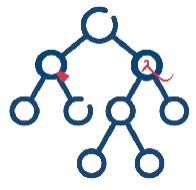
\includegraphics[height=1.0cm]{msca_logo.png}}%
    \end{center}

    \vspace{0.6cm}

    % Main title with Q logos on sides (with clickable links)
    \begin{center}
        \begin{minipage}{0.1\textwidth}
            \centering
            \href{https://quantlet.com}{
\includegraphics[height=1.1cm]{ql_logo.png}}
        \end{minipage}%
        \begin{minipage}{0.78\textwidth}
            \centering
            {\LARGE\bfseries\usebeamercolor[fg]{title}\inserttitle}

            \vspace{0.3cm}

            {\usebeamerfont{subtitle}\usebeamercolor[fg]{title}\insertsubtitle}
        \end{minipage}%
        \begin{minipage}{0.1\textwidth}
            \centering
            \href{https://quantinar.com}{
\includegraphics[height=1.1cm]{qr_logo.png}}
        \end{minipage}
    \end{center}

    \vspace{0.6cm}

    % Authors (left aligned)
    \hspace{0.5cm}{\usebeamerfont{author}\insertauthor}

    \vspace{0.3cm}

    % Institute/Affiliations (left aligned)
    \hspace{0.5cm}\begin{minipage}[t]{0.9\textwidth}
        \raggedright\small\insertinstitute
    \end{minipage}
}

%=============================================================================
% THEOREM ENVIRONMENTS
%=============================================================================
\theoremstyle{definition}
\setbeamertemplate{theorems}[numbered]
\ifdefined\sfmlang
\newtheorem{defn}{Definiție}
\newtheorem{thm}{Teoremă}
\newtheorem{prop}{Propoziție}
\newtheorem{rmk}{Observație}
\else
\newtheorem{defn}{Definition}
\newtheorem{thm}{Theorem}
\newtheorem{prop}{Proposition}
\newtheorem{rmk}{Remark}
\fi

%=============================================================================
% CENTRED MINIPAGE (no extra vertical space)
%=============================================================================
\newenvironment{cminipage}[1]{%
    \par\noindent\hfill\begin{minipage}{#1}\ignorespaces
}{%
    \end{minipage}\hfill\null\par
}

%=============================================================================
% CUSTOM COMMANDS
%=============================================================================
\newcommand{\E}{\mathbb{E}}
\newcommand{\Var}{\text{Var}}
\newcommand{\Cov}{\text{Cov}}
\newcommand{\Corr}{\text{Corr}}
\newcommand{\R}{\mathbb{R}}
\newcommand{\N}{\mathbb{N}}
\newcommand{\Z}{\mathbb{Z}}
\newcommand{\B}{\mathbf{B}}
\newcommand{\imark}{\textcolor{MainBlue}{\textbullet}}
\newcommand{\RMSE}{\text{RMSE}}
\newcommand{\MAE}{\text{MAE}}
\newcommand{\MAPE}{\text{MAPE}}

 se definește
%   \newcommand{\coursename}{Statistics of Financial Markets}      (EN)
%   \newcommand{\coursename}{Statistica piețelor financiare}       (RO)  și  \def\sfmlang{ro}
% Fișierele .tex se află în EN/Courses, EN/Seminars, RO/Cursuri, RO/Seminarii (două niveluri sub rădăcină).
% Deck-urile sînt generate de latex/build_chapterN.py / build_seminarN.py (vezi latex/sfm_build.py).

\documentclass[9pt, aspectratio=169, t]{beamer}
\providecommand{\coursename}{Statistics of Financial Markets}

% Ensure content fits on slides
\setbeamersize{text margin left=8mm, text margin right=8mm}

%=============================================================================
% THEME AND STYLE CONFIGURATION
%=============================================================================
\usetheme{default}
% Using default theme for clean header/footer control

% Color Palette (matching Redispatch PDF)
\definecolor{MainBlue}{RGB}{26, 58, 110}
\definecolor{AccentBlue}{RGB}{26, 58, 110}
\definecolor{IDAred}{RGB}{205, 0, 0}
\definecolor{DarkGray}{RGB}{51, 51, 51}
\definecolor{MediumGray}{RGB}{128, 128, 128}
\definecolor{LightGray}{RGB}{248, 248, 248}
\definecolor{VeryLightGray}{RGB}{235, 235, 235}
\definecolor{KeynoteGray}{RGB}{218, 218, 218}
\definecolor{SectionGray}{RGB}{120, 120, 120}
\definecolor{FooterGray}{RGB}{100, 100, 100}
\definecolor{Crimson}{RGB}{220, 53, 69}
\definecolor{Forest}{RGB}{46, 125, 50}
\definecolor{Amber}{RGB}{181, 133, 63}
\definecolor{Orange}{RGB}{230, 126, 34}
\definecolor{Purple}{RGB}{142, 68, 173}

% Gradient background (exact Keynote 315° gradient: white to RGB 218,218,218)
\setbeamertemplate{background}{%
    \begin{tikzpicture}[remember picture, overlay]
        \shade[shading=axis, shading angle=315,
        top color=white, bottom color=KeynoteGray]
        (current page.south west) rectangle (current page.north east);
    \end{tikzpicture}%
}
% Fallback solid color for compatibility
\setbeamercolor{background canvas}{bg=}

\setbeamercolor{palette primary}{bg=MainBlue, fg=white}
\setbeamercolor{palette secondary}{bg=MainBlue!85, fg=white}
\setbeamercolor{palette tertiary}{bg=MainBlue!70, fg=white}
\setbeamercolor{structure}{fg=MainBlue}
\setbeamercolor{title}{fg=IDAred}
\setbeamercolor{frametitle}{fg=IDAred, bg=}
\setbeamercolor{block title}{bg=MainBlue, fg=white}
\setbeamercolor{block body}{bg=VeryLightGray, fg=DarkGray}
\setbeamercolor{block title alerted}{bg=Crimson, fg=white}
\setbeamercolor{block body alerted}{bg=Crimson!8, fg=DarkGray}
\setbeamercolor{block title example}{bg=Forest, fg=white}
\setbeamercolor{block body example}{bg=Forest!8, fg=DarkGray}
\setbeamercolor{item}{fg=MainBlue}

% Footer colors (override Madrid theme blue)
\setbeamercolor{author in head/foot}{fg=FooterGray, bg=}
\setbeamercolor{title in head/foot}{fg=FooterGray, bg=}
\setbeamercolor{date in head/foot}{fg=FooterGray, bg=}
\setbeamercolor{section in head/foot}{fg=FooterGray, bg=}
\setbeamercolor{subsection in head/foot}{fg=FooterGray, bg=}

% Bullet styles (apply everywhere including blocks)
\setbeamertemplate{itemize item}{\color{MainBlue}$\boxdot$}
\setbeamertemplate{itemize subitem}{\color{MainBlue}$\blacktriangleright$}
\setbeamertemplate{itemize subsubitem}{\color{MainBlue}\tiny$\bullet$}
\setbeamertemplate{itemize/enumerate body begin}{\normalsize}
\setbeamertemplate{itemize/enumerate subbody begin}{\normalsize}

% Item spacing - compact style
\setlength{\leftmargini}{10pt}       % Level 1: minimal indent
\setlength{\leftmarginii}{10pt}      % Level 2: minimal additional indent
% Compact list spacing (zero extra space before/after lists in blocks)
\makeatletter
\def\@listi{\leftmargin\leftmargini \topsep 0pt \parsep 0pt \itemsep 0pt}
\def\@listii{\leftmargin\leftmarginii \topsep 0pt \parsep 0pt \itemsep 0pt}
\makeatother

\setbeamertemplate{navigation symbols}{}

%=============================================================================
% CUSTOM HEADLINE
%=============================================================================
\setbeamertemplate{headline}{%
    \vskip10pt%
    \hbox to \paperwidth{%
        \hskip0.5cm%
        {\small\color{FooterGray}\renewcommand{\hyperlink}[2]{##2}\insertsectionhead}%
        \hfill%
        \textcolor{FooterGray}{\small\insertframenumber}%
        \hskip0.5cm%
    }%
    \vskip4pt%
    {\color{FooterGray}\hrule height 0.4pt}%
}

%=============================================================================
% CUSTOM FOOTER
%=============================================================================
\usepackage{fontawesome5}

\setbeamertemplate{footline}{%
    {\color{FooterGray}\hrule height 0.4pt}%
    \vskip4pt%
    \hbox to \paperwidth{%
        \hskip0.5cm%
        \textcolor{FooterGray}{\small\coursename}%
        \hfill%
        \raisebox{-0.1em}{%
            \begin{tikzpicture}[x=0.08em, y=0.08em, line width=0.4pt]
                \draw[FooterGray] (0,3) -- (1,4) -- (2,3.5) -- (3,5) -- (4,4) -- (5,6) -- (6,5.5) -- (7,4) -- (8,5) -- (9,7) -- (10,6) -- (11,5) -- (12,6.5) -- (13,8) -- (14,7) -- (15,6) -- (16,7.5) -- (17,9) -- (18,8) -- (19,7) -- (20,8.5) -- (21,10) -- (22,9) -- (23,8) -- (24,9.5);
            \end{tikzpicture}%
        }%
        \hskip0.5cm%
    }%
    \vskip6pt%
}

%=============================================================================
% PACKAGES
%=============================================================================
\usepackage[utf8]{inputenc}
\DeclareUnicodeCharacter{03B1}{\ensuremath{\alpha}}
\usepackage[T1]{fontenc}
\usepackage{amsmath, amssymb, amsthm}
\usepackage{mathtools}
\usepackage{bm}
\usepackage{tikz}
\usetikzlibrary{arrows.meta, positioning, shapes, calc, decorations.pathreplacing, shadings}
\usepackage{booktabs}
\usepackage{multirow}
\usepackage{array}
\usepackage{graphicx}
\usepackage{hyperref}
\usepackage{colortbl}
\usepackage{listings}
\lstset{language=Python, basicstyle=\ttfamily\scriptsize, keywordstyle=\color{MainBlue}\bfseries,
  commentstyle=\color{Forest}, stringstyle=\color{Crimson}, breaklines=true,
  frame=none, backgroundcolor=\color{VeryLightGray}, xleftmargin=2mm}
\hypersetup{colorlinks=true, linkcolor=MainBlue, urlcolor=MainBlue}
\graphicspath{{../../logos/}{../../charts/}{../../photos/}}
\usepackage{xcolor}
\hfuzz=2pt  % Suppress tiny overfull warnings (<2pt)
\vfuzz=2pt  % Suppress tiny vertical overfull warnings (<2pt)

%=============================================================================
% QUANTLET COMMANDS
%   \quantlet{<displayed name>}{<url>}       (generic, compatible with the older SFM decks)
%   \sfmquantlet{Ch_05}{SFM_ch5_garch}       -> https://github.com/danpele/SFM/tree/main/Quantlets/Ch_05/SFM_ch5_garch
%   \qlurl{<folder>} is defined per chapter by the generator (Quantlets/Ch_NN/<folder>)
%=============================================================================
\newcommand{\sfmrepo}{https://github.com/danpele/SFM}
\newcommand{\sfmqlbase}{https://github.com/danpele/SFM/tree/main/Quantlets}
\newcommand{\quantlet}[2]{%
    \hfill\href{#2}{%
        \raisebox{-0.15em}{
\includegraphics[height=0.7em]{ql_logo.png}}%
        \textcolor{MainBlue}{\tiny\ #1}%
    }%
}
\newcommand{\sfmquantlet}[2]{\quantlet{\detokenize{#2}}{\sfmqlbase/#1/#2}}

%=============================================================================
% NOTEBOOKS (Google Colab)
%   \colaburl{notebooks/EN/chapter5_seminar_notebook.ipynb} -> the Colab link of a file in the SFM repo
%   \nb: the chapter notebook (each seminar deck redefines it with \renewcommand)
%=============================================================================
\newcommand{\colaburl}[1]{https://colab.research.google.com/github/danpele/SFM/blob/main/#1}
\newcommand{\nb}{https://colab.research.google.com/github/danpele/SFM/tree/main/notebooks/EN}
\newcommand{\nbname}{notebooks/EN}

%=============================================================================
% SLIDE HELPERS (used by the generators; the same as in MFM)
%=============================================================================
% local font size for list bodies (the preamble forces \normalsize)
\newcommand{\itemsize}[1]{\setbeamertemplate{itemize/enumerate body begin}{#1}\setbeamertemplate{itemize/enumerate subbody begin}{#1}}
\newcommand{\intitle}[1]{{\hypersetup{urlcolor=white}#1}}   % white links inside coloured title bars
\newcommand{\imgcap}[1]{{\scriptsize #1}\\[0.5mm]}          % caption under a photo
\newcommand{\imgcredit}[2]{{\tiny\color{FooterGray}\href{#1}{#2}}}   % image credit: source URL, author/licence
\newcommand{\aiprompt}[1]{{\ttfamily\color{MainBlue}#1}}     % a prompt to an AI assistant

%=============================================================================
% SEMINARS: student version by default; the instructor wrapper *_solutions.tex sets \solutionstrue
%=============================================================================
\makeatletter\@ifundefined{ifsolutions}{\expandafter\newif\csname ifsolutions\endcsname}{}\makeatother
\newcommand{\solonly}[1]{\ifsolutions #1\fi}
\newcommand{\propsub}{\ifsolutions\else\framesubtitle{\ifdefined\sfmlang Rezolvarea se discută la seminar\else Solution discussed in class\fi}\fi}

%=============================================================================
% APPENDIX AND CHAPTER LINKS (latex/appendix_links.py writes the calls; it also re-declares these
% macros before \begin{document}, so the decks compile with or without this preamble block)
%=============================================================================
\providecommand{\sfmapplink}[3]{\hypertarget{#2}{}\hyperlink{#1}{\beamergotobutton{#3}}}
\providecommand{\sfmappback}[2]{\begin{tikzpicture}[remember picture,overlay]\node[anchor=south east] at ([xshift=-3mm,yshift=7mm]current page.south east){\hyperlink{#1}{\beamerreturnbutton{#2}}};\end{tikzpicture}}
\providecommand{\sfmchlink}[2]{\href{#1}{#2}}
\providecommand{\sfmchlinkt}[2]{\href{#1}{\usebeamercolor[fg]{frametitle}#2}}

%=============================================================================
% QUANTINAR COMMAND: link către un curs Quantinar (subiecte avansate)
%=============================================================================
\newcommand{\quantinar}[2]{%
    \href{#2}{%
        \raisebox{-0.15em}{
\includegraphics[height=0.8em]{qr_logo.png}}%
        \textcolor{MainBlue}{\scriptsize\ #1}%
    }%
}

%=============================================================================
% CUSTOM TITLE PAGE
%=============================================================================
\defbeamertemplate*{title page}{hybrid}[1][]
{
    \vspace{0.2cm}
    % Logos row - top header (with clickable links)
    \begin{center}
        \href{https://www.ase.ro}{
\includegraphics[height=1.0cm]{ase_logo.png}}\hspace{0.3cm}%
        \href{https://theida.net}{
\includegraphics[height=1.0cm]{ida_logo.png}}\hspace{0.3cm}%
        \href{https://blockchain-research-center.com}{
\includegraphics[height=1.0cm]{brc_logo.png}}\hspace{0.3cm}%
        \href{https://www.ai4efin.ase.ro}{
\includegraphics[height=1.0cm]{ai4efin_logo.png}}\hspace{0.3cm}%
        \href{https://ipe.ro/new}{
\includegraphics[height=1.0cm]{acad_logo.png}}\hspace{0.3cm}%
        \href{https://www.digital-finance-msca.com}{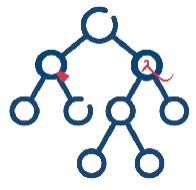
\includegraphics[height=1.0cm]{msca_logo.png}}%
    \end{center}

    \vspace{0.6cm}

    % Main title with Q logos on sides (with clickable links)
    \begin{center}
        \begin{minipage}{0.1\textwidth}
            \centering
            \href{https://quantlet.com}{
\includegraphics[height=1.1cm]{ql_logo.png}}
        \end{minipage}%
        \begin{minipage}{0.78\textwidth}
            \centering
            {\LARGE\bfseries\usebeamercolor[fg]{title}\inserttitle}

            \vspace{0.3cm}

            {\usebeamerfont{subtitle}\usebeamercolor[fg]{title}\insertsubtitle}
        \end{minipage}%
        \begin{minipage}{0.1\textwidth}
            \centering
            \href{https://quantinar.com}{
\includegraphics[height=1.1cm]{qr_logo.png}}
        \end{minipage}
    \end{center}

    \vspace{0.6cm}

    % Authors (left aligned)
    \hspace{0.5cm}{\usebeamerfont{author}\insertauthor}

    \vspace{0.3cm}

    % Institute/Affiliations (left aligned)
    \hspace{0.5cm}\begin{minipage}[t]{0.9\textwidth}
        \raggedright\small\insertinstitute
    \end{minipage}
}

%=============================================================================
% THEOREM ENVIRONMENTS
%=============================================================================
\theoremstyle{definition}
\setbeamertemplate{theorems}[numbered]
\ifdefined\sfmlang
\newtheorem{defn}{Definiție}
\newtheorem{thm}{Teoremă}
\newtheorem{prop}{Propoziție}
\newtheorem{rmk}{Observație}
\else
\newtheorem{defn}{Definition}
\newtheorem{thm}{Theorem}
\newtheorem{prop}{Proposition}
\newtheorem{rmk}{Remark}
\fi

%=============================================================================
% CENTRED MINIPAGE (no extra vertical space)
%=============================================================================
\newenvironment{cminipage}[1]{%
    \par\noindent\hfill\begin{minipage}{#1}\ignorespaces
}{%
    \end{minipage}\hfill\null\par
}

%=============================================================================
% CUSTOM COMMANDS
%=============================================================================
\newcommand{\E}{\mathbb{E}}
\newcommand{\Var}{\text{Var}}
\newcommand{\Cov}{\text{Cov}}
\newcommand{\Corr}{\text{Corr}}
\newcommand{\R}{\mathbb{R}}
\newcommand{\N}{\mathbb{N}}
\newcommand{\Z}{\mathbb{Z}}
\newcommand{\B}{\mathbf{B}}
\newcommand{\imark}{\textcolor{MainBlue}{\textbullet}}
\newcommand{\RMSE}{\text{RMSE}}
\newcommand{\MAE}{\text{MAE}}
\newcommand{\MAPE}{\text{MAPE}}

 se definește
%   \newcommand{\coursename}{Statistics of Financial Markets}      (EN)
%   \newcommand{\coursename}{Statistica piețelor financiare}       (RO)  și  \def\sfmlang{ro}
% Fișierele .tex se află în EN/Courses, EN/Seminars, RO/Cursuri, RO/Seminarii (două niveluri sub rădăcină).
% Deck-urile sînt generate de latex/build_chapterN.py / build_seminarN.py (vezi latex/sfm_build.py).

\documentclass[9pt, aspectratio=169, t]{beamer}
\providecommand{\coursename}{Statistics of Financial Markets}

% Ensure content fits on slides
\setbeamersize{text margin left=8mm, text margin right=8mm}

%=============================================================================
% THEME AND STYLE CONFIGURATION
%=============================================================================
\usetheme{default}
% Using default theme for clean header/footer control

% Color Palette (matching Redispatch PDF)
\definecolor{MainBlue}{RGB}{26, 58, 110}
\definecolor{AccentBlue}{RGB}{26, 58, 110}
\definecolor{IDAred}{RGB}{205, 0, 0}
\definecolor{DarkGray}{RGB}{51, 51, 51}
\definecolor{MediumGray}{RGB}{128, 128, 128}
\definecolor{LightGray}{RGB}{248, 248, 248}
\definecolor{VeryLightGray}{RGB}{235, 235, 235}
\definecolor{KeynoteGray}{RGB}{218, 218, 218}
\definecolor{SectionGray}{RGB}{120, 120, 120}
\definecolor{FooterGray}{RGB}{100, 100, 100}
\definecolor{Crimson}{RGB}{220, 53, 69}
\definecolor{Forest}{RGB}{46, 125, 50}
\definecolor{Amber}{RGB}{181, 133, 63}
\definecolor{Orange}{RGB}{230, 126, 34}
\definecolor{Purple}{RGB}{142, 68, 173}

% Gradient background (exact Keynote 315° gradient: white to RGB 218,218,218)
\setbeamertemplate{background}{%
    \begin{tikzpicture}[remember picture, overlay]
        \shade[shading=axis, shading angle=315,
        top color=white, bottom color=KeynoteGray]
        (current page.south west) rectangle (current page.north east);
    \end{tikzpicture}%
}
% Fallback solid color for compatibility
\setbeamercolor{background canvas}{bg=}

\setbeamercolor{palette primary}{bg=MainBlue, fg=white}
\setbeamercolor{palette secondary}{bg=MainBlue!85, fg=white}
\setbeamercolor{palette tertiary}{bg=MainBlue!70, fg=white}
\setbeamercolor{structure}{fg=MainBlue}
\setbeamercolor{title}{fg=IDAred}
\setbeamercolor{frametitle}{fg=IDAred, bg=}
\setbeamercolor{block title}{bg=MainBlue, fg=white}
\setbeamercolor{block body}{bg=VeryLightGray, fg=DarkGray}
\setbeamercolor{block title alerted}{bg=Crimson, fg=white}
\setbeamercolor{block body alerted}{bg=Crimson!8, fg=DarkGray}
\setbeamercolor{block title example}{bg=Forest, fg=white}
\setbeamercolor{block body example}{bg=Forest!8, fg=DarkGray}
\setbeamercolor{item}{fg=MainBlue}

% Footer colors (override Madrid theme blue)
\setbeamercolor{author in head/foot}{fg=FooterGray, bg=}
\setbeamercolor{title in head/foot}{fg=FooterGray, bg=}
\setbeamercolor{date in head/foot}{fg=FooterGray, bg=}
\setbeamercolor{section in head/foot}{fg=FooterGray, bg=}
\setbeamercolor{subsection in head/foot}{fg=FooterGray, bg=}

% Bullet styles (apply everywhere including blocks)
\setbeamertemplate{itemize item}{\color{MainBlue}$\boxdot$}
\setbeamertemplate{itemize subitem}{\color{MainBlue}$\blacktriangleright$}
\setbeamertemplate{itemize subsubitem}{\color{MainBlue}\tiny$\bullet$}
\setbeamertemplate{itemize/enumerate body begin}{\normalsize}
\setbeamertemplate{itemize/enumerate subbody begin}{\normalsize}

% Item spacing - compact style
\setlength{\leftmargini}{10pt}       % Level 1: minimal indent
\setlength{\leftmarginii}{10pt}      % Level 2: minimal additional indent
% Compact list spacing (zero extra space before/after lists in blocks)
\makeatletter
\def\@listi{\leftmargin\leftmargini \topsep 0pt \parsep 0pt \itemsep 0pt}
\def\@listii{\leftmargin\leftmarginii \topsep 0pt \parsep 0pt \itemsep 0pt}
\makeatother

\setbeamertemplate{navigation symbols}{}

%=============================================================================
% CUSTOM HEADLINE
%=============================================================================
\setbeamertemplate{headline}{%
    \vskip10pt%
    \hbox to \paperwidth{%
        \hskip0.5cm%
        {\small\color{FooterGray}\renewcommand{\hyperlink}[2]{##2}\insertsectionhead}%
        \hfill%
        \textcolor{FooterGray}{\small\insertframenumber}%
        \hskip0.5cm%
    }%
    \vskip4pt%
    {\color{FooterGray}\hrule height 0.4pt}%
}

%=============================================================================
% CUSTOM FOOTER
%=============================================================================
\usepackage{fontawesome5}

\setbeamertemplate{footline}{%
    {\color{FooterGray}\hrule height 0.4pt}%
    \vskip4pt%
    \hbox to \paperwidth{%
        \hskip0.5cm%
        \textcolor{FooterGray}{\small\coursename}%
        \hfill%
        \raisebox{-0.1em}{%
            \begin{tikzpicture}[x=0.08em, y=0.08em, line width=0.4pt]
                \draw[FooterGray] (0,3) -- (1,4) -- (2,3.5) -- (3,5) -- (4,4) -- (5,6) -- (6,5.5) -- (7,4) -- (8,5) -- (9,7) -- (10,6) -- (11,5) -- (12,6.5) -- (13,8) -- (14,7) -- (15,6) -- (16,7.5) -- (17,9) -- (18,8) -- (19,7) -- (20,8.5) -- (21,10) -- (22,9) -- (23,8) -- (24,9.5);
            \end{tikzpicture}%
        }%
        \hskip0.5cm%
    }%
    \vskip6pt%
}

%=============================================================================
% PACKAGES
%=============================================================================
\usepackage[utf8]{inputenc}
\DeclareUnicodeCharacter{03B1}{\ensuremath{\alpha}}
\usepackage[T1]{fontenc}
\usepackage{amsmath, amssymb, amsthm}
\usepackage{mathtools}
\usepackage{bm}
\usepackage{tikz}
\usetikzlibrary{arrows.meta, positioning, shapes, calc, decorations.pathreplacing, shadings}
\usepackage{booktabs}
\usepackage{multirow}
\usepackage{array}
\usepackage{graphicx}
\usepackage{hyperref}
\usepackage{colortbl}
\usepackage{listings}
\lstset{language=Python, basicstyle=\ttfamily\scriptsize, keywordstyle=\color{MainBlue}\bfseries,
  commentstyle=\color{Forest}, stringstyle=\color{Crimson}, breaklines=true,
  frame=none, backgroundcolor=\color{VeryLightGray}, xleftmargin=2mm}
\hypersetup{colorlinks=true, linkcolor=MainBlue, urlcolor=MainBlue}
\graphicspath{{../../logos/}{../../charts/}{../../photos/}}
\usepackage{xcolor}
\hfuzz=2pt  % Suppress tiny overfull warnings (<2pt)
\vfuzz=2pt  % Suppress tiny vertical overfull warnings (<2pt)

%=============================================================================
% QUANTLET COMMANDS
%   \quantlet{<displayed name>}{<url>}       (generic, compatible with the older SFM decks)
%   \sfmquantlet{Ch_05}{SFM_ch5_garch}       -> https://github.com/danpele/SFM/tree/main/Quantlets/Ch_05/SFM_ch5_garch
%   \qlurl{<folder>} is defined per chapter by the generator (Quantlets/Ch_NN/<folder>)
%=============================================================================
\newcommand{\sfmrepo}{https://github.com/danpele/SFM}
\newcommand{\sfmqlbase}{https://github.com/danpele/SFM/tree/main/Quantlets}
\newcommand{\quantlet}[2]{%
    \hfill\href{#2}{%
        \raisebox{-0.15em}{
\includegraphics[height=0.7em]{ql_logo.png}}%
        \textcolor{MainBlue}{\tiny\ #1}%
    }%
}
\newcommand{\sfmquantlet}[2]{\quantlet{\detokenize{#2}}{\sfmqlbase/#1/#2}}

%=============================================================================
% NOTEBOOKS (Google Colab)
%   \colaburl{notebooks/EN/chapter5_seminar_notebook.ipynb} -> the Colab link of a file in the SFM repo
%   \nb: the chapter notebook (each seminar deck redefines it with \renewcommand)
%=============================================================================
\newcommand{\colaburl}[1]{https://colab.research.google.com/github/danpele/SFM/blob/main/#1}
\newcommand{\nb}{https://colab.research.google.com/github/danpele/SFM/tree/main/notebooks/EN}
\newcommand{\nbname}{notebooks/EN}

%=============================================================================
% SLIDE HELPERS (used by the generators; the same as in MFM)
%=============================================================================
% local font size for list bodies (the preamble forces \normalsize)
\newcommand{\itemsize}[1]{\setbeamertemplate{itemize/enumerate body begin}{#1}\setbeamertemplate{itemize/enumerate subbody begin}{#1}}
\newcommand{\intitle}[1]{{\hypersetup{urlcolor=white}#1}}   % white links inside coloured title bars
\newcommand{\imgcap}[1]{{\scriptsize #1}\\[0.5mm]}          % caption under a photo
\newcommand{\imgcredit}[2]{{\tiny\color{FooterGray}\href{#1}{#2}}}   % image credit: source URL, author/licence
\newcommand{\aiprompt}[1]{{\ttfamily\color{MainBlue}#1}}     % a prompt to an AI assistant

%=============================================================================
% SEMINARS: student version by default; the instructor wrapper *_solutions.tex sets \solutionstrue
%=============================================================================
\makeatletter\@ifundefined{ifsolutions}{\expandafter\newif\csname ifsolutions\endcsname}{}\makeatother
\newcommand{\solonly}[1]{\ifsolutions #1\fi}
\newcommand{\propsub}{\ifsolutions\else\framesubtitle{\ifdefined\sfmlang Rezolvarea se discută la seminar\else Solution discussed in class\fi}\fi}

%=============================================================================
% APPENDIX AND CHAPTER LINKS (latex/appendix_links.py writes the calls; it also re-declares these
% macros before \begin{document}, so the decks compile with or without this preamble block)
%=============================================================================
\providecommand{\sfmapplink}[3]{\hypertarget{#2}{}\hyperlink{#1}{\beamergotobutton{#3}}}
\providecommand{\sfmappback}[2]{\begin{tikzpicture}[remember picture,overlay]\node[anchor=south east] at ([xshift=-3mm,yshift=7mm]current page.south east){\hyperlink{#1}{\beamerreturnbutton{#2}}};\end{tikzpicture}}
\providecommand{\sfmchlink}[2]{\href{#1}{#2}}
\providecommand{\sfmchlinkt}[2]{\href{#1}{\usebeamercolor[fg]{frametitle}#2}}

%=============================================================================
% QUANTINAR COMMAND: link către un curs Quantinar (subiecte avansate)
%=============================================================================
\newcommand{\quantinar}[2]{%
    \href{#2}{%
        \raisebox{-0.15em}{
\includegraphics[height=0.8em]{qr_logo.png}}%
        \textcolor{MainBlue}{\scriptsize\ #1}%
    }%
}

%=============================================================================
% CUSTOM TITLE PAGE
%=============================================================================
\defbeamertemplate*{title page}{hybrid}[1][]
{
    \vspace{0.2cm}
    % Logos row - top header (with clickable links)
    \begin{center}
        \href{https://www.ase.ro}{
\includegraphics[height=1.0cm]{ase_logo.png}}\hspace{0.3cm}%
        \href{https://theida.net}{
\includegraphics[height=1.0cm]{ida_logo.png}}\hspace{0.3cm}%
        \href{https://blockchain-research-center.com}{
\includegraphics[height=1.0cm]{brc_logo.png}}\hspace{0.3cm}%
        \href{https://www.ai4efin.ase.ro}{
\includegraphics[height=1.0cm]{ai4efin_logo.png}}\hspace{0.3cm}%
        \href{https://ipe.ro/new}{
\includegraphics[height=1.0cm]{acad_logo.png}}\hspace{0.3cm}%
        \href{https://www.digital-finance-msca.com}{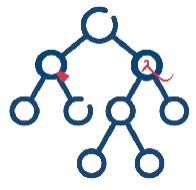
\includegraphics[height=1.0cm]{msca_logo.png}}%
    \end{center}

    \vspace{0.6cm}

    % Main title with Q logos on sides (with clickable links)
    \begin{center}
        \begin{minipage}{0.1\textwidth}
            \centering
            \href{https://quantlet.com}{
\includegraphics[height=1.1cm]{ql_logo.png}}
        \end{minipage}%
        \begin{minipage}{0.78\textwidth}
            \centering
            {\LARGE\bfseries\usebeamercolor[fg]{title}\inserttitle}

            \vspace{0.3cm}

            {\usebeamerfont{subtitle}\usebeamercolor[fg]{title}\insertsubtitle}
        \end{minipage}%
        \begin{minipage}{0.1\textwidth}
            \centering
            \href{https://quantinar.com}{
\includegraphics[height=1.1cm]{qr_logo.png}}
        \end{minipage}
    \end{center}

    \vspace{0.6cm}

    % Authors (left aligned)
    \hspace{0.5cm}{\usebeamerfont{author}\insertauthor}

    \vspace{0.3cm}

    % Institute/Affiliations (left aligned)
    \hspace{0.5cm}\begin{minipage}[t]{0.9\textwidth}
        \raggedright\small\insertinstitute
    \end{minipage}
}

%=============================================================================
% THEOREM ENVIRONMENTS
%=============================================================================
\theoremstyle{definition}
\setbeamertemplate{theorems}[numbered]
\ifdefined\sfmlang
\newtheorem{defn}{Definiție}
\newtheorem{thm}{Teoremă}
\newtheorem{prop}{Propoziție}
\newtheorem{rmk}{Observație}
\else
\newtheorem{defn}{Definition}
\newtheorem{thm}{Theorem}
\newtheorem{prop}{Proposition}
\newtheorem{rmk}{Remark}
\fi

%=============================================================================
% CENTRED MINIPAGE (no extra vertical space)
%=============================================================================
\newenvironment{cminipage}[1]{%
    \par\noindent\hfill\begin{minipage}{#1}\ignorespaces
}{%
    \end{minipage}\hfill\null\par
}

%=============================================================================
% CUSTOM COMMANDS
%=============================================================================
\newcommand{\E}{\mathbb{E}}
\newcommand{\Var}{\text{Var}}
\newcommand{\Cov}{\text{Cov}}
\newcommand{\Corr}{\text{Corr}}
\newcommand{\R}{\mathbb{R}}
\newcommand{\N}{\mathbb{N}}
\newcommand{\Z}{\mathbb{Z}}
\newcommand{\B}{\mathbf{B}}
\newcommand{\imark}{\textcolor{MainBlue}{\textbullet}}
\newcommand{\RMSE}{\text{RMSE}}
\newcommand{\MAE}{\text{MAE}}
\newcommand{\MAPE}{\text{MAPE}}



\newcommand{\qlurl}[1]{https://github.com/danpele/SFM/tree/main/Quantlets/Ch_13/#1}
\renewcommand{\nb}{\colaburl{notebooks/EN/chapter13_seminar_notebook.ipynb}}
\renewcommand{\nbname}{chapter13\_seminar\_notebook.ipynb}
% left column: full width in the student version, narrower next to the solution
\newcommand{\taskw}{\ifsolutions 0.47\textwidth\else 0.96\textwidth\fi}
\newcommand{\solw}{\ifsolutions 0.49\textwidth\else 0pt\fi}

% Clickable citations (DOIs verified via Crossref)

\newcommand{\refFHH}{\href{https://doi.org/10.1007/978-3-030-13751-9}{Franke, Härdle \& Hafner (2019)}}
\newcommand{\refBHL}{\href{https://doi.org/10.1007/978-3-642-33929-5}{Borak, Härdle \& López-Cabrera (2013)}}
\newcommand{\refISL}{\href{https://doi.org/10.1007/978-3-031-38747-0}{James et al.\ (2023)}}
\newcommand{\refHTF}{\href{https://doi.org/10.1007/978-0-387-84858-7}{Hastie, Tibshirani \& Friedman (2009)}}
\newcommand{\refBreimanTC}{\href{https://doi.org/10.1214/ss/1009213726}{Breiman (2001a)}}
\newcommand{\refBreiman}{\href{https://doi.org/10.1023/A:1010933404324}{Breiman (2001b)}}
\newcommand{\refFriedman}{\href{https://doi.org/10.1214/aos/1013203451}{Friedman (2001)}}
\newcommand{\refHK}{\href{https://doi.org/10.1080/00401706.1970.10488634}{Hoerl \& Kennard (1970)}}
\newcommand{\refTib}{\href{https://doi.org/10.1111/j.2517-6161.1996.tb02080.x}{Tibshirani (1996)}}
\newcommand{\refRosenblatt}{\href{https://doi.org/10.1037/h0042519}{Rosenblatt (1958)}}
\newcommand{\refHSW}{\href{https://doi.org/10.1016/0893-6080(89)90020-8}{Hornik, Stinchcombe \& White (1989)}}
\newcommand{\refRHW}{\href{https://doi.org/10.1038/323533a0}{Rumelhart, Hinton \& Williams (1986)}}
\newcommand{\refCorsi}{\href{https://doi.org/10.1093/jjfinec/nbp001}{Corsi (2009)}}
\newcommand{\refGK}{\href{https://doi.org/10.1086/296072}{Garman \& Klass (1980)}}
\newcommand{\refPatton}{\href{https://doi.org/10.1016/j.jeconom.2010.03.034}{Patton (2011)}}
\newcommand{\refDM}{\href{https://doi.org/10.1080/07350015.1995.10524599}{Diebold \& Mariano (1995)}}
\newcommand{\refCT}{\href{https://doi.org/10.1093/rfs/hhm055}{Campbell \& Thompson (2008)}}
\newcommand{\refWG}{\href{https://doi.org/10.1093/rfs/hhm014}{Welch \& Goyal (2008)}}
\newcommand{\refKB}{\href{https://doi.org/10.2307/1913643}{Koenker \& Bassett (1978)}}
\newcommand{\refCAViaR}{\href{https://doi.org/10.1198/073500104000000370}{Engle \& Manganelli (2004)}}
\newcommand{\refKupiec}{\href{https://doi.org/10.3905/jod.1995.407942}{Kupiec (1995)}}
\newcommand{\refChris}{\href{https://doi.org/10.2307/2527341}{Christoffersen (1998)}}
\newcommand{\refBLdP}{\href{https://doi.org/10.3905/jpm.2014.40.5.094}{Bailey \& López de Prado (2014)}}
\newcommand{\refHLZ}{\href{https://doi.org/10.1093/rfs/hhv059}{Harvey, Liu \& Zhu (2016)}}
\newcommand{\refWhite}{\href{https://doi.org/10.1111/1468-0262.00152}{White (2000)}}
\newcommand{\refLdP}{\href{https://www.wiley.com/en-us/Advances+in+Financial+Machine+Learning-p-9781119482086}{López de Prado (2018)}}
\newcommand{\refBHK}{\href{https://doi.org/10.1016/j.csda.2017.11.003}{Bergmeir, Hyndman \& Koo (2018)}}
\newcommand{\refGKX}{\href{https://doi.org/10.1093/rfs/hhaa009}{Gu, Kelly \& Xiu (2020)}}
\newcommand{\refKX}{\href{https://doi.org/10.1561/0500000064}{Kelly \& Xiu (2023)}}
\newcommand{\refCSV}{\href{https://doi.org/10.1093/jjfinec/nbac020}{Christensen, Siggaard \& Veliyev (2023)}}
\newcommand{\refLL}{\href{https://proceedings.neurips.cc/paper/2017/hash/8a20a8621978632d76c43dfd28b67767-Abstract.html}{Lundberg \& Lee (2017)}}
\newcommand{\refEngle}{\href{https://doi.org/10.2307/1912773}{Engle (1982)}}
\newcommand{\refBoll}{\href{https://doi.org/10.1016/0304-4076(86)90063-1}{Bollerslev (1986)}}
\newcommand{\refWang}{\href{https://doi.org/10.1038/s41586-023-06221-2}{Wang et al.\ (2023)}}
\newcommand{\refPeleA}{\href{https://doi.org/10.1080/1351847X.2021.1960403}{Pele et al.\ (2023)}}
\newcommand{\refPeleB}{\href{https://doi.org/10.3390/math14132316}{Pele \& Mazurencu-Marinescu-Pele (2026)}}
\newcommand{\refSFEa}{\href{https://github.com/QuantLet/SFE/tree/master/QID-3386-SFEnnarch}{SFEnnarch}}
\newcommand{\refSFEb}{\href{https://github.com/QuantLet/SFE/tree/master/QID-3387-SFEnnjpyusd}{SFEnnjpyusd}}

\title[Statistica piețelor financiare]{Statistica piețelor financiare}
\subtitle{Seminarul 13: Învățare automată\ifsolutions\ (versiunea profesorului)\fi}
\author[D.T. Pele]{Daniel Traian PELE}
\institute{Academia de Studii Economice din București\\
IDA Institute Digital Assets\\
Blockchain Research Center\\
AI4EFin Artificial Intelligence for Energy Finance\\
Academia Română, Institutul de Prognoză Economică\\
MSCA Digital Finance}
\date{}

%=============================================================================
\providecommand{\sfmapplink}[3]{\hypertarget{#2}{}\hyperlink{#1}{\beamergotobutton{#3}}}  % APPLINKS-MACROS
\providecommand{\sfmappback}[2]{\begin{tikzpicture}[remember picture,overlay]\node[anchor=south east] at ([xshift=-3mm,yshift=7mm]current page.south east){\hyperlink{#1}{\beamerreturnbutton{#2}}};\end{tikzpicture}}  % APPLINKS-MACROS
\providecommand{\sfmchlink}[2]{\href{#1}{#2}}  % APPLINKS-MACROS
\providecommand{\sfmchlinkt}[2]{\href{#1}{\usebeamercolor[fg]{frametitle}#2}}  % APPLINKS-MACROS
\begin{document}
%=============================================================================

{
\setbeamertemplate{headline}{}
\setbeamertemplate{footline}{}
\begin{frame}[noframenumbering]
    \titlepage
\end{frame}
}
% BEGIN-ACRONYMS (generat de latex/acronyms.py; nu editati manual)
\begin{frame}{Acronime folosite în acest material}
\setbeamertemplate{itemize/enumerate body begin}{\tiny}
\begin{columns}[T]
\begin{column}{0.49\textwidth}
\begin{itemize}\setlength{\itemsep}{0pt}
    \item \textbf{AI}: Artificial Intelligence (inteligență artificială)
    \item \textbf{AUC}: Area Under the (ROC) Curve (aria de sub curba ROC)
    \item \textbf{BET}: Bucharest Exchange Trading (index) — indicele de referință al Bursei de Valori București
    \item \textbf{BVB}: Bursa de Valori București
    \item \textbf{DM}: Diebold–Mariano (test) — testul Diebold–Mariano de comparare a prognozelor
    \item \textbf{EODHD}: EOD Historical Data (market-data provider) — furnizor de date de piață
    \item \textbf{GB}: Gradient Boosting (boosting pe gradient)
    \item \textbf{HAR}: Heterogeneous AutoRegressive (model) — model autoregresiv heterogen
    \item \textbf{HS}: Historical Simulation (simularea istorică)
    \item \textbf{ML}: Machine Learning (învățare automată)
    \item \textbf{MLP}: MultiLayer Perceptron (perceptron multistrat)
    \item \textbf{MSE}: Mean Squared Error (eroarea pătratică medie)
    \item \textbf{OLS}: Ordinary Least Squares (metoda celor mai mici pătrate)
\end{itemize}
\end{column}
\begin{column}{0.49\textwidth}
\begin{itemize}\setlength{\itemsep}{0pt}
    \item \textbf{OMV}: Österreichische Mineralölverwaltung (Administrația austriacă a uleiurilor minerale, grupul OMV)
    \item \textbf{QGB}: Quantile Gradient Boosting (gradient boosting cu pierdere cuantilică)
    \item \textbf{QLIKE}: Quasi-LIKElihood (loss function) — funcția de pierdere de tip cvasi-verosimilitate
    \item \textbf{QR}: Quantile Regression (regresie cuantilică)
    \item \textbf{RF}: Random Forest (pădure aleatoare)
    \item \textbf{ROC}: Receiver Operating Characteristic (curve) — curba caracteristică de operare
    \item \textbf{SPX}: S\&P 500 index (ticker symbol) — indicele S\&P 500 (simbolul de tranzacționare)
    \item \textbf{SSE}: Sum of Squared Errors (suma pătratelor erorilor)
    \item \textbf{VIX}: CBOE Volatility IndeX (indicele de volatilitate CBOE)
\end{itemize}
\end{column}
\end{columns}
\end{frame}
% END-ACRONYMS

\begin{frame}{Întrebarea de azi și traseul}
\itemsize{\small}
\begin{itemize}
    \item \textbf{Întrebarea}: cînd bate o metodă flexibilă de predicție un model simplu pe date financiare și cum o testăm fără să ne înșelăm singuri?
    \begin{itemize}
        \item seminarul are loc \textbf{înaintea} Cursului 13: secțiunea „Noțiuni necesare azi” dă toate definițiile folosite în cerințe
    \end{itemize}
    \item Traseul
    \begin{itemize}
        \item Partea A: deplasare și varianță, o împărțire a unui arbore, ridge și lasso într-o dimensiune, designuri walk-forward și cu purging, pe hîrtie
        \item Partea B: prognoze de volatilitate, semnul randamentelor și VaR 1\% pe date reale, fiecare cu o întrebare de interpretare
        \item Partea C: o întrebare deschisă pentru proiect și un răspuns AI de verificat
    \end{itemize}
    \item Notebook-ul de azi: \href{\nb}{deschideți notebook-ul seminarului în Google Colab}; fiecare cerință indică secțiunea din notebook
    \item Seminarul are rol de exercițiu și nu se notează; rezolvările cerințelor [Propus] se discută la seminar
\end{itemize}
\end{frame}

\begin{frame}{Harta exercițiilor}
\itemsize{\small}
\begin{center}
\footnotesize
\begin{tabular}{>{\raggedright\arraybackslash}p{1.1cm}>{\raggedright\arraybackslash}p{7.5cm}>{\raggedright\arraybackslash}p{1.9cm}>{\raggedright\arraybackslash}p{1.4cm}}
\toprule
\textbf{Cerința} & \textbf{Întrebarea} & \textbf{Tipul} & \textbf{Model} \\
\midrule
A1, A2 & deplasarea, varianța și eroarea așteptată din cinci eșantioane de antrenare & Rezolvat, Propus & A1 \\
A3, A4 & cea mai bună împărțire a unui arbore de regresie, pas cu pas & Rezolvat, Propus & A3 \\
A5, A6 & ridge și lasso cu o singură variabilă & Rezolvat, Propus & A5 \\
A7, A8 & un design walk-forward; un K-fold cu purging și embargo & Rezolvat, Propus & A7 \\
B1, B2 & prognoze de volatilitate: S\&P 500 (ziua următoare), DAX (săptămîna următoare) & Rezolvat, Propus & B1 \\
B3, B4 & semnul randamentelor zilnice: DAX; TLV și SNP & Rezolvat, Propus & B3 \\
B5, B6 & VaR 1\% pentru DAX prin regresie cuantilică și quantile boosting & Rezolvat, Propus & B5 \\
C1, C2 & ajută S\&P 500 la prognoza volatilității BET? ce este greșit într-un răspuns AI? & Propus & B2, A7 \\
\bottomrule
\end{tabular}
\end{center}
\begin{itemize}
    \item \textbf{[Rezolvat]}: rezolvarea completă în slide-uri și în notebook, un model de urmat; \textbf{[Propus]}: îl rezolvați voi, după model
\end{itemize}
\end{frame}

\begin{frame}{Datele folosite}
\itemsize{\small}
\begin{center}
\footnotesize
\begin{tabular}{llll}
\toprule
\textbf{Seria} & \textbf{Sursa} & \textbf{Prețurile folosite} & \textbf{Perioada} \\
\midrule
S\&P 500 & EODHD & deschidere, maxim, minim, închidere & 2008--2026 \\
DAX & EODHD & deschidere, maxim, minim, închidere & 2006--2026 \\
BET & EODHD & închidere & 2008--2026 \\
Banca Transilvania (TLV), OMV Petrom (SNP) & EODHD & închidere ajustată & 2010--2026 \\
\bottomrule
\end{tabular}
\end{center}
\begin{itemize}
    \item Randamente logaritmice zilnice în \%: $r_t = 100\,(\ln P_t - \ln P_{t-1})$; variabila proxy zilnică a varianței $v_t$ din deschidere, maxim, minim și închidere (\sfmchlink{https://danpele.github.io/SFM/RO/Cursuri/capitol8_estimatori_volatilitate.pdf}{Capitolul 8}); ultima zi este 18 septembrie 2026
    \item În notebook: \texttt{rv\_frame('dax')}, \texttt{walk\_forward(...)}, \texttt{rv\_metrics(...)}, \texttt{sign\_walk\_forward('dax')}, \texttt{var\_backtest(...)} (scikit-learn); nu este nevoie de cont sau de cheie
\end{itemize}
\end{frame}


%=============================================================================
\section{Noțiuni necesare azi}
%=============================================================================

\begin{frame}{Noțiuni necesare azi (1/5): învățarea din date}
\itemsize{\small}
\begin{itemize}
    \item \textbf{Machine learning} (ML, învățare automată): alegem din date o regulă de predicție $\hat f$ astfel încît $\hat f(x)$ să fie aproape de $y$ pe date \textbf{noi}
    \begin{itemize}
        \item $x_t$: \textbf{variabilele explicative} (features) cunoscute la închiderea zilei $t$; $y_t$: \textbf{ținta}; pierderea: de exemplu eroarea pătratică $(y - \hat y)^2$, MSE fiind media ei
    \end{itemize}
    \item \textbf{Overfitting}: o eroare mică pe datele de antrenare și o eroare mare pe date noi
    \begin{itemize}
        \item un \textbf{hiperparametru} (adîncimea arborelui, penalizarea) controlează flexibilitatea și se alege pe date nefolosite la estimare
    \end{itemize}
    \item \textbf{Deplasare--varianță}: dacă $y = f(x) + \varepsilon$, $\mathrm{Var}(\varepsilon) = \sigma^2$, iar $\hat f$ este estimat pe un eșantion de antrenare aleator
    \begin{itemize}
        \item $E[(y_0 - \hat f(x_0))^2] = (E\hat f(x_0) - f(x_0))^2 + \mathrm{Var}(\hat f(x_0)) + \sigma^2$: deplasare$^2$ + varianță + zgomot
        \item din $M$ eșantioane de antrenare: deplasarea $= \bar f - f$, varianța $= \frac1M\sum_m (\hat f_m - \bar f)^2$, cu $\bar f$ prognoza medie
    \end{itemize}
\end{itemize}
\end{frame}

\begin{frame}{Noțiuni necesare azi (2/5): validarea pentru serii de timp}
\itemsize{\small}
\begin{itemize}
    \item \textbf{Walk-forward}: antrenăm pe trecut, testăm pe blocul următor (aici: un an calendaristic), reestimăm și avansăm
    \begin{itemize}
        \item fereastra extinsă: eșantionul de antrenare păstrează toate zilele anterioare
    \end{itemize}
    \item \textbf{Purging}: o țintă $y_t$ construită din zilele $t+1, \dots, t+h$ se suprapune cu blocul de test dacă $t$ este una dintre ultimele $h$ zile de antrenare: le eliminăm
    \begin{itemize}
        \item \textbf{embargo}: la K-fold eliminăm și cîteva zile de antrenare imediat după blocul de test
    \end{itemize}
    \item \textbf{Look-ahead bias}: o variabilă folosește informație încă necunoscută la momentul $t$ (prețuri viitoare, medii pe tot eșantionul)
    \begin{itemize}
        \item \textbf{leakage} (scurgerea de informație): informația despre țintele de test ajunge în antrenare; \textbf{K-fold aleator} (partiții amestecate) o produce cînd țintele se suprapun
    \end{itemize}
\end{itemize}
\end{frame}

\begin{frame}{Noțiuni necesare azi (3/5): ridge și lasso}
\itemsize{\small}
\begin{itemize}
    \item \textbf{Ridge}: minimizăm $\sum_t (y_t - x_t^\top\beta)^2 + \lambda\sum_j \beta_j^2$; \textbf{lasso}: $\dots + \lambda\sum_j |\beta_j|$ ($\lambda \ge 0$: penalizarea)
    \begin{itemize}
        \item ambele schimbă o deplasare mică pe o varianță mai mică; lasso anulează exact unii coeficienți
    \end{itemize}
    \item \textbf{O singură variabilă centrată}, $S_{xx} = \sum_t x_t^2$, $S_{xy} = \sum_t x_ty_t$, fără termen liber
    \begin{itemize}
        \item OLS: $\hat\beta = S_{xy}/S_{xx}$; ridge: $\hat\beta = S_{xy}/(S_{xx} + \lambda)$
        \item lasso: $\hat\beta = \mathrm{sign}(S_{xy})\max(|S_{xy}| - \lambda/2, 0)/S_{xx}$ (pragul moale, soft thresholding)
    \end{itemize}
    \item Standardizăm variabilele cu media și abaterea standard din eșantionul de antrenare înainte de penalizare
\end{itemize}
\end{frame}

\begin{frame}{Noțiuni necesare azi (4/5): arbori, ansambluri și rețele}
\itemsize{\small}
\begin{itemize}
    \item \textbf{Arborele de regresie}: împărțim la $x_j \le s$; fiecare frunză prezice media valorilor $y$ din ea; alegem $(j, s)$ care minimizează
    \begin{itemize}
        \item $\mathrm{SSE}(s) = \sum_{x_j \le s}(y - \bar y_L)^2 + \sum_{x_j > s}(y - \bar y_R)^2$; candidați: mijloacele dintre valorile ordonate
    \end{itemize}
    \item \textbf{Random forest} (RF): media multor arbori adînci, fiecare crescut pe un eșantion bootstrap, cu submulțimi aleatoare de variabile
    \begin{itemize}
        \item \textbf{gradient boosting} (GB): arbori mici adăugați pe rînd, fiecare estimat pe reziduurile curente și scalat cu o rată de învățare
    \end{itemize}
    \item \textbf{MLP} (multilayer perceptron, perceptron multistrat): $\hat y = c + \sum_k v_k\, g(b_k + w_k^\top x)$, cu $g(z) = \max(0, z)$ (ReLU)
    \begin{itemize}
        \item reperul \textbf{HAR} (heterogeneous autoregressive, autoregresiv heterogen): OLS al logaritmului varianței viitoare pe logaritmul varianței din ultima zi, săptămînă și lună
    \end{itemize}
\end{itemize}
\end{frame}

\begin{frame}{Noțiuni necesare azi (5/5): evaluarea}
\itemsize{\footnotesize}
\begin{itemize}
    \item $R^2$ în afara eșantionului față de un reper $\tilde y$: $R^2_{OOS} = 1 - \sum(y_t - \hat y_t)^2/\sum(y_t - \tilde y_t)^2$; QLIKE: $L_t = \mathrm{RV}_t/\hat h_t + \ln\hat h_t$
    \begin{itemize}
        \item testul \textbf{DM} (Diebold--Mariano) pentru $d_t = L_t^A - L_t^B$: $\bar d/\mathrm{se}(\bar d) \sim N(0, 1)$; negativ: $A$ este mai bun
    \end{itemize}
    \item Clasificare: acuratețea comparată cu \textbf{reperul clasei majoritare} $\mathrm{acc}_0$; $z = (\widehat{\mathrm{acc}} - \mathrm{acc}_0)/\sqrt{\mathrm{acc}_0(1 - \mathrm{acc}_0)/n}$
    \begin{itemize}
        \item AUC: aria de sub curba ROC (\sfmchlink{https://danpele.github.io/SFM/RO/Cursuri/capitol12_modele_scoring.pdf}{Capitolul 12}); 0,5 = nicio abilitate
    \end{itemize}
    \item \textbf{Regresia cuantilică}: $\hat q_\alpha(x) = x^\top\hat\beta_\alpha$ minimizează $\sum_t \rho_\alpha(y_t - x_t^\top\beta)$, $\rho_\alpha(u) = u(\alpha - \mathbf{1}\{u < 0\})$
    \begin{itemize}
        \item VaR 1\% $= -\hat q_{0{,}01}$, o pierdere pozitivă; backtesting cu Kupiec (rata) și Christoffersen (independența), \sfmchlink{https://danpele.github.io/SFM/RO/Cursuri/capitol10_var_es_backtesting.pdf}{Capitolul 10}
    \end{itemize}
\end{itemize}
\end{frame}


%=============================================================================
\section{Partea A: calcule pe hîrtie}
%=============================================================================

\begin{frame}{A1: deplasarea și varianța unui arbore puțin adînc [Rezolvat]}
\itemsize{\scriptsize}
\begin{columns}[T]
\begin{column}{0.47\textwidth}
\begin{block}{Cerință}
\begin{itemize}
    \item Într-un punct $x_0$, valoarea reală este $f(x_0) = 2{,}0$ și $\sigma^2 = 0{,}25$. Un arbore de adîncime 1 estimat pe cinci eșantioane de antrenare prognozează 1,6; 1,7; 1,5; 1,8; 1,6.
    \item 1. Calculați prognoza medie și deplasarea.
    \item 2. Calculați varianța celor cinci prognoze (împărțiți la 5).
    \item 3. Calculați eroarea pătratică așteptată în $x_0$.
    \item Raportați: patru valori și o frază.
\end{itemize}
\end{block}
\end{column}
\begin{column}{0.49\textwidth}
\begin{exampleblock}{Rezolvare}
\begin{itemize}
    \item 1. $\bar f = 8{,}2/5 = 1{,}640$; deplasarea $= 1{,}640 - 2 = -0{,}360$
    \item 2. $[(-0{,}04)^2 + 0{,}06^2 + (-0{,}14)^2 + 0{,}16^2 + (-0{,}04)^2]/5 = 0{,}0104$
    \item 3. $0{,}1296 + 0{,}0104 + 0{,}25 = 0{,}390$
    \item Arborele puțin adînc este stabil, dar sistematic prea jos: eroarea lui este în principal deplasare la pătrat.
\end{itemize}
\end{exampleblock}
\end{column}
\end{columns}
\end{frame}

\begin{frame}{A2: deplasarea și varianța unui arbore adînc [Propus]}
\propsub
\itemsize{\scriptsize}
\begin{columns}[T]
\begin{column}{\taskw}
\begin{block}{Cerință}
\begin{itemize}
    \item Același punct și același zgomot ca în A1. Un arbore de adîncime 10, pe aceleași cinci eșantioane, prognozează 2,6; 1,4; 2,3; 1,7; 2,2. Model: A1.
    \item 1. Calculați prognoza medie, deplasarea și varianța.
    \item 2. Calculați eroarea pătratică așteptată.
    \item 3. Decideți ce arbore ați folosi în $x_0$.
    \item Raportați: patru valori și o frază.
\end{itemize}
\end{block}
\end{column}
\begin{column}{\solw}
\solonly{%
\begin{exampleblock}{Rezolvare}
\begin{itemize}
    \item 1. $\bar f = 2{,}040$; deplasarea $= 0{,}040$; varianța $= 0{,}1864$
    \item 2. $0{,}0016 + 0{,}1864 + 0{,}25 = 0{,}438$
    \item 3. Arborele puțin adînc: $0{,}390 < 0{,}438$.
    \item Arborele adînc este aproape nedeplasat, dar varianța lui costă mai mult decît deplasarea arborelui puțin adînc.
\end{itemize}
\end{exampleblock}
}
\end{column}
\end{columns}
\end{frame}

\begin{frame}{A3: o împărțire a unui arbore de regresie [Rezolvat]}
\itemsize{\scriptsize}
\begin{columns}[T]
\begin{column}{0.47\textwidth}
\begin{block}{Cerință}
\begin{itemize}
    \item Opt zile: $x$ = randamentul absolut de ieri (\%), $y$ = variabila proxy a varianței de azi:
    \item $x$: 0,2; 0,4; 0,5; 0,9; 1,1; 1,6; 2,0; 2,8; $y$: 0,5; 0,7; 0,6; 1,0; 1,4; 2,2; 2,6; 3,4
    \item 1. Calculați media lui $y$ și SSE fără împărțire.
    \item 2. Pentru fiecare împărțire candidată, calculați mediile celor două frunze și SSE total.
    \item 3. Alegeți cea mai bună împărțire și ponderea din SSE pe care o elimină.
    \item Raportați: tabelul, împărțirea și o frază.
\end{itemize}
\end{block}
\end{column}
\begin{column}{0.49\textwidth}
\begin{exampleblock}{Rezolvare}
\begin{center}
\tiny
\begin{tabular}{rrrr}
\toprule
$s$ & $\bar y_L$ & $\bar y_R$ & SSE \\
\midrule
$0{,}30$ & $0{,}500$ & $1{,}700$ & $6{,}740$ \\
$0{,}45$ & $0{,}600$ & $1{,}867$ & $5{,}593$ \\
$0{,}70$ & $0{,}600$ & $2{,}120$ & $3{,}668$ \\
$1{,}00$ & $0{,}700$ & $2{,}400$ & $2{,}220$ \\
$1{,}35$ & $0{,}840$ & $2{,}733$ & $1{,}279$ \\
$1{,}80$ & $1{,}067$ & $3{,}000$ & $2{,}393$ \\
$2{,}40$ & $1{,}286$ & $3{,}400$ & $4{,}089$ \\
\bottomrule
\end{tabular}
\end{center}
\begin{itemize}
    \item $\bar y = 1{,}550$, SSE $= 8{,}000$; cea mai bună $s = 1{,}35$: frunzele $0{,}840$ și $2{,}733$, SSE $= 0{,}532 + 0{,}747 = 1{,}279$
    \item împărțirea elimină $1 - 1{,}279/8{,}000 = 0{,}840$ din SSE: mișcări mari ieri, varianță mare azi
\end{itemize}
\end{exampleblock}
\end{column}
\end{columns}
\end{frame}

\begin{frame}{A4: o împărțire după indicele de volatilitate [Propus]}
\propsub
\itemsize{\scriptsize}
\begin{columns}[T]
\begin{column}{\taskw}
\begin{block}{Cerință}
\begin{itemize}
    \item Opt luni: $x$ = nivelul VIX la sfîrșitul lunii, $y$ = volatilitatea realizată din luna următoare (\% pe zi). Model: A3.
    \item $x$: 12, 14, 15, 17, 21, 24, 30, 38; $y$: 0,8; 0,9; 0,7; 1,1; 1,5; 1,4; 2,6; 3,0
    \item 1. Calculați SSE fără împărțire și pentru fiecare împărțire candidată.
    \item 2. Alegeți cea mai bună împărțire și precizați prognozele celor două frunze.
    \item 3. Calculați ponderea din SSE eliminată de împărțire.
    \item Raportați: tabelul, trei valori și o frază.
\end{itemize}
\end{block}
\end{column}
\begin{column}{\solw}
\solonly{%
\begin{exampleblock}{Rezolvare}
\begin{center}
\tiny
\begin{tabular}{rrrr}
\toprule
$s$ & $\bar y_L$ & $\bar y_R$ & SSE \\
\midrule
$13{,}0$ & $0{,}800$ & $1{,}600$ & $4{,}560$ \\
$14{,}5$ & $0{,}850$ & $1{,}717$ & $3{,}993$ \\
$16{,}0$ & $0{,}800$ & $1{,}920$ & $2{,}768$ \\
$19{,}0$ & $0{,}875$ & $2{,}125$ & $1{,}995$ \\
$22{,}5$ & $1{,}000$ & $2{,}333$ & $1{,}787$ \\
$27{,}0$ & $1{,}067$ & $2{,}800$ & $0{,}613$ \\
$34{,}0$ & $1{,}286$ & $3{,}000$ & $2{,}549$ \\
\bottomrule
\end{tabular}
\end{center}
\begin{itemize}
    \item SSE fără împărțire $5{,}120$; cea mai bună $s = 27{,}0$: frunzele $1{,}067$ și $2{,}800$, SSE $= 0{,}613$, o pondere eliminată de $0{,}880$
    \item Un VIX ridicat anunță o lună volatilă; arborele găsește pragul fără un model liniar.
\end{itemize}
\end{exampleblock}
}
\end{column}
\end{columns}
\end{frame}

\begin{frame}{A5: ridge cu o singură variabilă [Rezolvat]}
\itemsize{\scriptsize}
\begin{columns}[T]
\begin{column}{0.47\textwidth}
\begin{block}{Cerință}
\begin{itemize}
    \item O singură variabilă centrată, cu $S_{xx} = 50$ și $S_{xy} = 20$; fără termen liber.
    \item 1. Calculați coeficientul OLS.
    \item 2. Calculați coeficientul ridge și factorul de contracție $S_{xx}/(S_{xx} + \lambda)$ pentru $\lambda = 10$ și $\lambda = 50$.
    \item 3. Explicați ce se întîmplă cînd $\lambda \to \infty$.
    \item Raportați: cinci valori și o frază.
\end{itemize}
\end{block}
\end{column}
\begin{column}{0.49\textwidth}
\begin{exampleblock}{Rezolvare}
\begin{itemize}
    \item 1. $\hat\beta^{OLS} = 20/50 = 0{,}40$
    \item 2. $\lambda = 10$: $20/60 = 0{,}333$, factorul $0{,}833$; $\lambda = 50$: $20/100 = 0{,}20$, factorul $0{,}50$
    \item 3. Coeficientul tinde la 0, dar nu devine niciodată 0.
    \item Ridge înmulțește coeficientul OLS cu un factor sub 1: contractă, nu selectează.
\end{itemize}
\end{exampleblock}
\end{column}
\end{columns}
\end{frame}

\begin{frame}{A6: lasso cu o singură variabilă [Propus]}
\propsub
\itemsize{\scriptsize}
\begin{columns}[T]
\begin{column}{\taskw}
\begin{block}{Cerință}
\begin{itemize}
    \item Aceleași date ca în A5: $S_{xx} = 50$, $S_{xy} = 20$. Model: A5.
    \item 1. Calculați coeficientul lasso pentru $\lambda = 10$, 30 și 50.
    \item 2. Găsiți cel mai mic $\lambda$ pentru care coeficientul este exact zero.
    \item 3. Comparați lasso cu rezultatele ridge din A5 pentru $\lambda = 50$.
    \item Raportați: patru valori și o frază.
\end{itemize}
\end{block}
\end{column}
\begin{column}{\solw}
\solonly{%
\begin{exampleblock}{Rezolvare}
\begin{itemize}
    \item 1. $(20 - 5)/50 = 0{,}30$; $(20 - 15)/50 = 0{,}10$; $\max(20 - 25, 0)/50 = 0{,}00$
    \item 2. $\lambda \ge 2|S_{xy}| = 40$
    \item 3. Pentru $\lambda = 50$, ridge păstrează $0{,}20$, iar lasso elimină variabila.
    \item Lasso scade o constantă din $|S_{xy}|$ (pragul moale): variabilele slabe dispar.
\end{itemize}
\end{exampleblock}
}
\end{column}
\end{columns}
\end{frame}

\begin{frame}{A7: un design walk-forward [Rezolvat]}
\itemsize{\scriptsize}
\begin{columns}[T]
\begin{column}{0.47\textwidth}
\begin{block}{Cerință}
\begin{itemize}
    \item Variabile zilnice S\&P 500 de la 8 aprilie 2008 la 18 septembrie 2026; ținta: varianța medie din următoarele 5 zile; reestimare în fiecare ianuarie din 2013.
    \item 1. Numărați partițiile evaluării walk-forward.
    \item 2. Pentru partiția din 2013, precizați ce zile de antrenare trebuie eliminate (purging) și de ce.
    \item 3. Explicați de ce nu este nevoie de embargo.
    \item 4. Explicați ce ar merge prost dacă modelul pentru 2013 ar fi calibrat prin 5-fold aleator pe 2008--2012.
    \item Raportați: două valori și trei fraze.
\end{itemize}
\end{block}
\end{column}
\begin{column}{0.49\textwidth}
\begin{exampleblock}{Rezolvare}
\begin{itemize}
    \item 1. O partiție pentru fiecare an 2013--2026: 14 partiții.
    \item 2. Ultimele 5 zile de antrenare (de la 24 decembrie 2012): țintele lor folosesc ianuarie 2013; partiția antrenează pe 1\,188 de zile, ultima fiind 21 decembrie 2012, și testează pe 252.
    \item 3. Toate zilele de antrenare sînt înaintea anului de test: nicio variabilă de antrenare nu folosește informație de test.
    \item 4. Partițiile aleatoare pun zile vecine, cu ținte suprapuse, în antrenare și în validare: hiperparametrii aleși recompensează memorarea, nu prognoza.
\end{itemize}
\end{exampleblock}
\end{column}
\end{columns}
\end{frame}

\begin{frame}{A8: K-fold cu purging și embargo [Propus]}
\propsub
\itemsize{\scriptsize}
\begin{columns}[T]
\begin{column}{\taskw}
\begin{block}{Cerință}
\begin{itemize}
    \item 2500 de zile, $K = 5$ blocuri în ordine temporală, o țintă care folosește următoarele 21 de zile, un embargo de 1\% din zile. Model: A7.
    \item 1. Calculați mărimea fiecărui bloc de test și a embargoului.
    \item 2. Calculați numărul de zile de antrenare cînd blocul de test este la mijloc.
    \item 3. Calculați-l cînd blocul de test este primul și cînd este ultimul.
    \item Raportați: patru valori și o frază.
\end{itemize}
\end{block}
\end{column}
\begin{column}{\solw}
\solonly{%
\begin{exampleblock}{Rezolvare}
\begin{itemize}
    \item 1. Blocul: $2500/5 = 500$ de zile; embargoul: $\lceil 25 \rceil = 25$ de zile
    \item 2. $2500 - 500 - 21 - 25 = 1\,954$ (21 eliminate înainte, 25 sub embargo după)
    \item 3. Primul bloc: doar embargoul, $1\,975$; ultimul bloc: doar purging-ul, $1\,979$
    \item Fiecare partiție interioară pierde 46 de zile; cu date zilnice este un preț mic pentru o validare onestă.
\end{itemize}
\end{exampleblock}
}
\end{column}
\end{columns}
\end{frame}


%=============================================================================
\section{Partea B: date reale, inferență și interpretare}
%=============================================================================

\begin{frame}{B1: volatilitatea S\&P 500 pentru ziua următoare [Rezolvat]}
\itemsize{\footnotesize}
\begin{itemize}
\item \textbf{Întrebarea}: prognozează un random forest varianța de mîine a S\&P 500 mai bine decît HAR?
\item \textbf{Date}: deschiderea, maximul, minimul și închiderea S\&P 500 din 2008; ținta: $\ln v_{t+1}$; variabilele: cele trei medii HAR
\item \textbf{Cerințe}
\begin{enumerate}
    \item Estimați HAR (OLS) și un random forest (300 de arbori, cel puțin 20 de zile într-o frunză) walk-forward, reestimînd în fiecare ianuarie din 2013.
    \item Calculați $R^2$ în afara eșantionului pentru ambele modele față de media de antrenare și pentru random forest față de HAR.
    \item Calculați QLIKE mediu pentru ambele și testul Diebold--Mariano al egalității QLIKE.
    \item Desenați diferența QLIKE pe ani.
    \item Interpretare: merită aici complexitatea random forest?
\end{enumerate}
\item \textbf{Raportați}: patru valori, un test cu p-valoarea lui, graficul și două fraze
\item Notebook: secțiunea B1
\end{itemize}
\end{frame}

\begin{frame}{B1: rezolvare [Rezolvat]}
\itemsize{\scriptsize}
\begin{center}
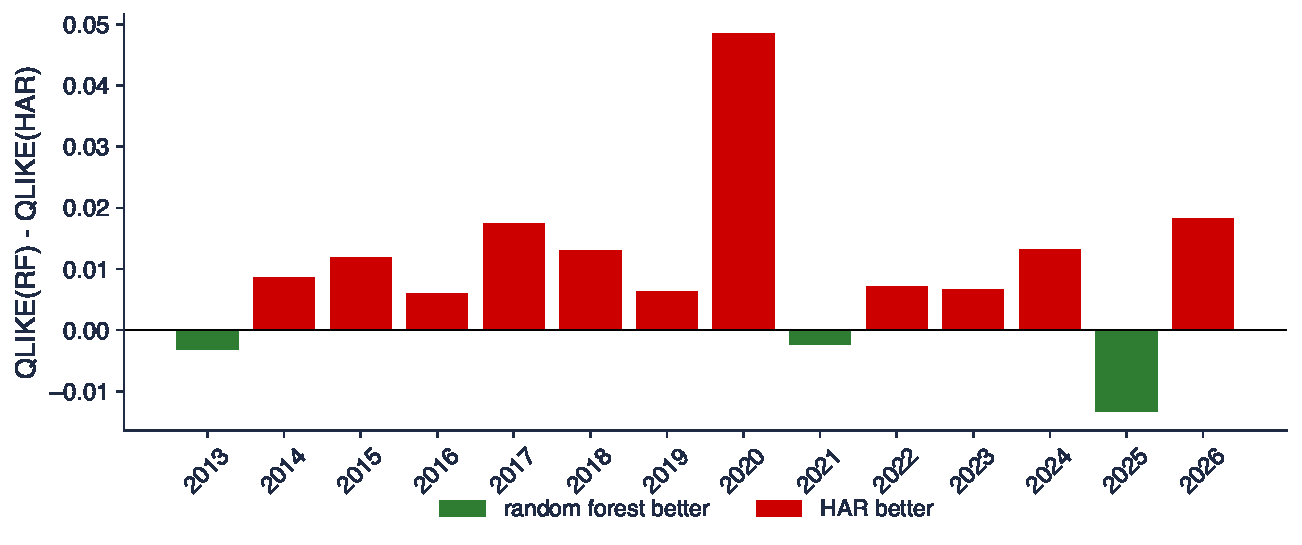
\includegraphics[width=0.96\textwidth,height=0.36\textheight,keepaspectratio]{ch13_sem_b1.pdf}
\end{center}
\vspace{-2mm}
\begin{itemize}
    \item 3\,448 de zile de la 2 ianuarie 2013; $R^2_{OOS}$ față de medie: HAR $54{,}8\%$, random forest $53{,}4\%$; random forest față de HAR: $-3{,}2\%$
    \item QLIKE: HAR $0{,}329$, random forest $0{,}339$; DM $= +2{,}65$ (p 0{,}008); random forest este mai bun doar în 3 din 14 ani
    \item Interpretare: nu: cu aceleași trei variabile, random forest este semnificativ mai slab decît HAR liniar; relația este aproape liniară în logaritmi, iar random forest adaugă varianță
\end{itemize}\sfmquantlet{Ch_13}{SFM_ch13_seminar}
\end{frame}

\begin{frame}{B2: volatilitatea săptămînală a DAX [Propus]}
\itemsize{\footnotesize}
\begin{itemize}
\item \textbf{Întrebarea}: bat lasso, random forest, gradient boosting sau un MLP modelul HAR pentru varianța DAX din săptămîna următoare? Model: B1.
\item \textbf{Date}: deschiderea, maximul, minimul și închiderea DAX din 2006; ținta: logaritmul mediei lui $v$ din următoarele 5 zile; 11 variabile (HAR, 4 decalaje, trimestrul, $r_t$, $\min(r_t, 0)$, $|r_t|$)
\item \textbf{Cerințe}
\begin{enumerate}
    \item Estimați cele cinci modele walk-forward din 2012, eliminînd ultimele 5 zile de antrenare.
    \item Calculați $R^2$ în afara eșantionului față de HAR și QLIKE mediu pentru fiecare model.
    \item Aplicați testul Diebold--Mariano pentru fiecare model față de HAR.
    \item Interpretare: ce model ați folosi pentru DAX?
\end{enumerate}
\item \textbf{Raportați}: un tabel și două fraze
\item Notebook: secțiunea B2
\end{itemize}
\end{frame}

\ifsolutions
\begin{frame}{B2: rezolvare [Propus]}
\itemsize{\footnotesize}
\begin{center}
\footnotesize
\begin{tabular}{lrrrr}
\toprule
Model & $R^2_{OOS}$ față de medie & $R^2_{OOS}$ față de HAR & QLIKE & DM (p) \\
\midrule
HAR & $54{,}3$ & -- & $1{,}031$ & -- \\
Lasso & $57{,}9$ & ${+7{,}8}$ & $1{,}022$ & ${-2{,}51}$ (0{,}012) \\
RF & $56{,}9$ & ${+5{,}7}$ & $1{,}027$ & ${-0{,}76}$ (0{,}450) \\
GB & $55{,}0$ & ${+1{,}5}$ & $1{,}032$ & ${+0{,}18}$ (0{,}855) \\
MLP & $58{,}3$ & ${+8{,}7}$ & $1{,}022$ & ${-2{,}05}$ (0{,}040) \\
\bottomrule
\end{tabular}
\end{center}
\begin{itemize}
    \item 3\,727 de zile de la 2 ianuarie 2012; $R^2_{OOS}$ în \%; DM față de HAR, negativ: mai bun decît HAR
    \item Interpretare: lasso ($+7{,}8\%$, p 0{,}012) sau MLP ($+8{,}7\%$, p 0{,}040); lasso este mai simplu, iar cîștigul lui este la fel de mare; arborii nu bat semnificativ HAR
\end{itemize}\sfmquantlet{Ch_13}{SFM_ch13_seminar}
\end{frame}
\fi

\begin{frame}{B3: semnul randamentelor DAX [Rezolvat]}
\itemsize{\footnotesize}
\begin{itemize}
\item \textbf{Întrebarea}: pot un logit sau un random forest să prezică dacă DAX crește mîine mai bine decît „mereu creștere”?
\item \textbf{Date}: închiderile DAX din 2000; ținta $\mathbf{1}\{r_{t+1} > 0\}$; variabilele: ultimele 5 randamente, sumele pe 5, 21 și 63 de zile, volatilitatea pe 21 și 63 de zile
\item \textbf{Cerințe}
\begin{enumerate}
    \item Estimați ambii clasificatori walk-forward din 2008, reestimînd în fiecare ianuarie.
    \item Calculați acuratețea fiecărui model și a reperului clasei majoritare.
    \item Testați fiecare acuratețe față de reper cu statistica $z$ și calculați AUC.
    \item Desenați acuratețea pe ani.
    \item Interpretare: are vreunul dintre modele o abilitate reală?
\end{enumerate}
\item \textbf{Raportați}: șase valori, graficul și două fraze
\item Notebook: secțiunea B3
\end{itemize}
\end{frame}

\begin{frame}{B3: rezolvare [Rezolvat]}
\itemsize{\scriptsize}
\begin{center}
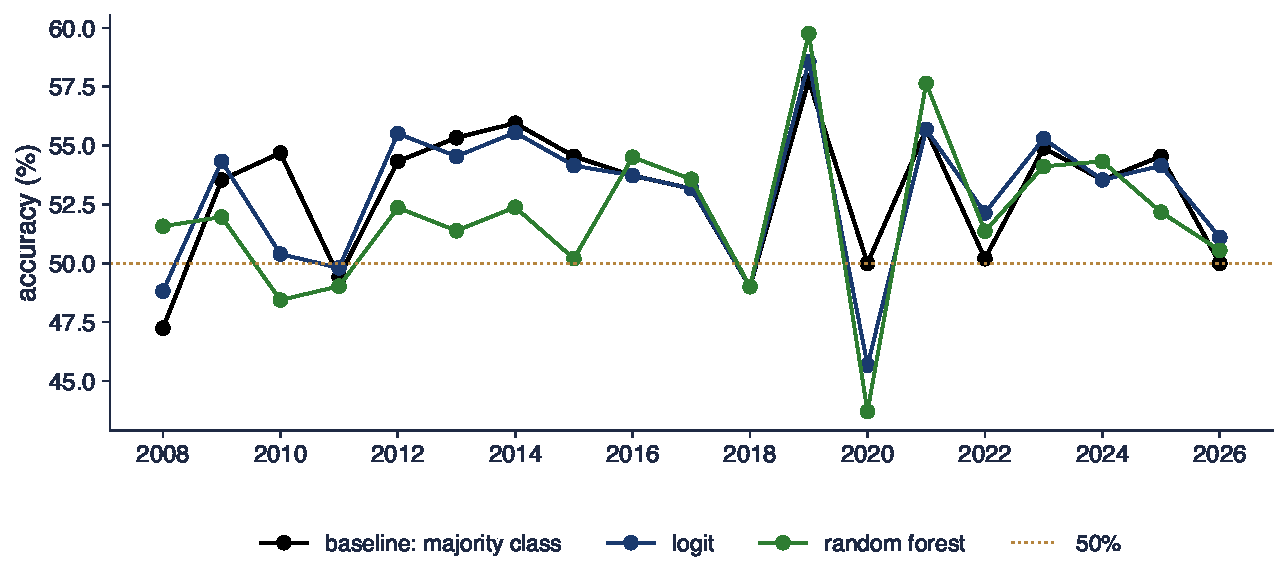
\includegraphics[width=0.96\textwidth,height=0.36\textheight,keepaspectratio]{ch13_sem_b3.pdf}
\end{center}
\vspace{-2mm}
\begin{itemize}
    \item $n = 4\,752$ de zile; zile de creștere 53{,}1\% = acuratețea reperului; logit 52{,}9\% ($z = -0{,}20$, p 0{,}839, AUC 0{,}507); random forest 52{,}0\% ($z = -1{,}45$, p 0{,}146, AUC 0{,}508)
    \item Logit prognozează „creștere” în 90\% din zile; random forest bate reperul în 8 din 19 ani, cam cît ar permite hazardul
    \item Interpretare: nu: ambele acurateți sînt la nivelul reperului sau sub el, iar AUC este aproape de 0,5; randamentele zilnice ale DAX sînt aproape imprevizibile (\sfmchlink{https://danpele.github.io/SFM/RO/Cursuri/capitol7_piete_eficiente_mers_aleator_vr.pdf}{Capitolul 7})
\end{itemize}\sfmquantlet{Ch_13}{SFM_ch13_seminar}
\end{frame}

\begin{frame}{B4: semnul a două acțiuni BVB [Propus]}
\itemsize{\footnotesize}
\begin{itemize}
\item \textbf{Întrebarea}: este semnul randamentelor Banca Transilvania și OMV Petrom mai ușor de prezis decît cel al DAX? Model: B3.
\item \textbf{Date}: închiderile ajustate TLV (fără 30--31 mai 2016) și SNP din 2010; variabilele din B3; prognoze din 2014
\item \textbf{Cerințe}
\begin{enumerate}
    \item Estimați logit, random forest și gradient boosting walk-forward din 2014.
    \item Calculați acuratețea, acuratețea reperului, statistica $z$ și AUC pentru fiecare acțiune și model.
    \item Interpretare: există mai multă predictibilitate la BVB decît la DAX?
\end{enumerate}
\item \textbf{Raportați}: un tabel și două fraze
\item Notebook: secțiunea B4
\end{itemize}
\end{frame}

\ifsolutions
\begin{frame}{B4: rezolvare [Propus]}
\itemsize{\footnotesize}
\begin{center}
\footnotesize
\begin{tabular}{lrlrrr}
\toprule
& reper (\%) & Model & acuratețe (\%) & $z$ (p) & AUC \\
\midrule
TLV & 54{,}0 & Logit & 52{,}9 & ${-1{,}23}$ (0{,}219) & 0{,}488 \\
 &  & RF & 52{,}2 & ${-1{,}94}$ (0{,}053) & 0{,}509 \\
 &  & GB & 52{,}8 & ${-1{,}38}$ (0{,}168) & 0{,}506 \\
\midrule
SNP & 51{,}2 & Logit & 51{,}9 & ${+0{,}82}$ (0{,}414) & 0{,}509 \\
 &  & RF & 52{,}2 & ${+1{,}04}$ (0{,}299) & 0{,}509 \\
 &  & GB & 51{,}9 & ${+0{,}78}$ (0{,}436) & 0{,}513 \\
\bottomrule
\end{tabular}
\end{center}
\begin{itemize}
    \item TLV: 2\,902 zile, SNP: 2\,905 zile, din 2014
    \item Interpretare: nu: nicio diferență nu este semnificativă la 5\%; modelele pentru SNP sînt puțin peste reper (random forest $+1{,}0$ puncte, p 0{,}299), cele pentru TLV sub el; AUC între 0{,}488 și 0{,}513
\end{itemize}\sfmquantlet{Ch_13}{SFM_ch13_seminar}
\end{frame}
\fi

\begin{frame}{B5: VaR 1\% pentru DAX prin regresie cuantilică [Rezolvat]}
\itemsize{\footnotesize}
\begin{itemize}
\item \textbf{Întrebarea}: dă o regresie cuantilică liniară pe variabile de volatilitate un VaR 1\% mai bun decît simularea istorică?
\item \textbf{Date}: DAX din 2006; ținta $r_{t+1}$; variabilele: $\sqrt{v_t}$, $\sqrt{\text{media lui } v}$ pe 5 și 22 de zile, $r_t$
\item \textbf{Cerințe}
\begin{enumerate}
    \item Estimați regresia cuantilică de nivel 1\% walk-forward din 2012 și luați VaR 1\% $= -\hat q_{0{,}01}$.
    \item Calculați VaR 1\% prin simulare istorică pe ultimele 500 de zile.
    \item Numărați depășirile, aplicați testele Kupiec și Christoffersen și calculați pierderea cuantilică medie.
    \item Desenați ambele prognoze VaR în 2020--2022.
    \item Interpretare: ce VaR ați raporta unui comitet de risc?
\end{enumerate}
\item \textbf{Raportați}: un tabel, graficul și două fraze
\item Notebook: secțiunea B5
\end{itemize}
\end{frame}

\begin{frame}{B5: rezolvare [Rezolvat]}
\itemsize{\scriptsize}
\begin{center}
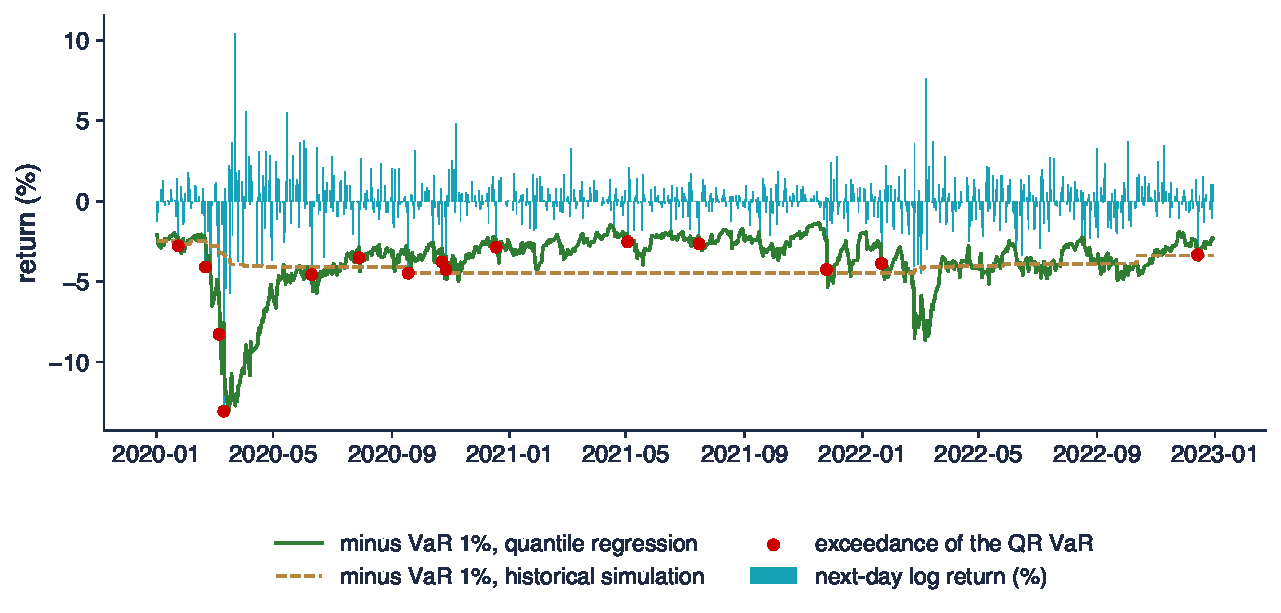
\includegraphics[width=0.96\textwidth,height=0.32\textheight,keepaspectratio]{ch13_sem_b5.pdf}
\end{center}
\vspace{-2mm}
\begin{center}
\scriptsize
\begin{tabular}{lrrrrr}
\toprule
Metoda & $x$ & rata (\%) & p Kupiec & p ind. & pierdere $\times 100$ \\
\midrule
QR & 39 & $1{,}05$ & 0{,}783 & 0{,}364 & $3{,}80$ \\
HS & 49 & $1{,}31$ & 0{,}066 & $<$\,0{,}001 & $4{,}75$ \\
\bottomrule
\end{tabular}
\end{center}
\begin{itemize}
    \item 3\,731 de zile de la 2 ianuarie 2012; ultima estimare: $\hat q_{0{,}01} = -0{,}472 -0{,}434\sqrt{v_t} -1{,}814\sqrt{v^{(w)}} -0{,}221\sqrt{v^{(m)}} +0{,}158 r_t$; VaR 1\% pe 17 septembrie 2026: 2{,}24\%
    \item Interpretare: regresia cuantilică: rată corectă, depășiri independente, pierdere mai mică; HS este depășit grupat (de 13 ori în 2020), deoarece o fereastră de 500 de zile reacționează lent
\end{itemize}\sfmquantlet{Ch_13}{SFM_ch13_seminar}
\end{frame}

\begin{frame}{B6: quantile gradient boosting pentru DAX [Propus]}
\itemsize{\footnotesize}
\begin{itemize}
\item \textbf{Întrebarea}: îmbunătățește un model cuantilic flexibil regresia cuantilică liniară din B5? Model: B5.
\item \textbf{Date}: ca în B5; gradient boosting cu pierderea cuantilică la 1\%, 300 de arbori de adîncime 2, rata de învățare 0,05, cel puțin 50 de zile într-o frunză
\item \textbf{Cerințe}
\begin{enumerate}
    \item Estimați quantile boosting walk-forward din 2012 și calculați VaR 1\%.
    \item Numărați depășirile, aplicați testele Kupiec și Christoffersen și calculați pierderea cuantilică.
    \item Interpretare: merită modelul flexibil la nivelul de 1\%?
\end{enumerate}
\item \textbf{Raportați}: un tabel și două fraze
\item Notebook: secțiunea B6
\end{itemize}
\end{frame}

\ifsolutions
\begin{frame}{B6: rezolvare [Propus]}
\itemsize{\footnotesize}
\begin{center}
\footnotesize
\begin{tabular}{lrrrrrr}
\toprule
Metoda & $x$ & rata (\%) & p Kupiec & p ind. & pierdere $\times 100$ & VaR mediu \\
\midrule
QR & 39 & $1{,}05$ & 0{,}783 & 0{,}364 & $3{,}80$ & $2{,}92$ \\
QGB & 71 & $1{,}90$ & $<$\,0{,}001 & 0{,}595 & $4{,}04$ & $2{,}71$ \\
\bottomrule
\end{tabular}
\end{center}
\begin{itemize}
    \item 3\,731 de zile; QGB: quantile gradient boosting
    \item Interpretare: nu: boosting este depășit mult prea des (1{,}90\%, p $<$\,0{,}001), iar pierderea lui este mai mare; la 1\% fiecare frunză vede foarte puține zile din coadă, deci modelul flexibil subestimează riscul
\end{itemize}\sfmquantlet{Ch_13}{SFM_ch13_seminar}
\end{frame}
\fi


%=============================================================================
\section{Partea C: întrebări deschise și critica unui răspuns AI}
%=============================================================================

\begin{frame}{C1: ajută S\&P 500 la prognoza volatilității BET? [Propus]}
\itemsize{\footnotesize}
\begin{itemize}
\item \textbf{Întrebarea}: BVB se închide înaintea bursei din New York; îmbunătățește volatilitatea S\&P 500 de ieri o prognoză HAR a varianței BET din săptămîna următoare?
\item \textbf{Date}: închiderile BET și S\&P 500 din 2008; proxy: randamentele zilnice la pătrat (BET nu are prețuri maxime și minime în datele noastre); modele: B1, B2
\item \textbf{Cerințe}
\begin{enumerate}
    \item Construiți variabilele HAR ale BET și variabilele HAR ale S\&P 500 de la închiderea precedentă din New York.
    \item Comparați HAR, HAR plus variabilele S\&P 500 (OLS) și un random forest pe toate variabilele, walk-forward din 2012.
    \item Calculați $R^2$ în afara eșantionului, QLIKE și testele Diebold--Mariano față de HAR.
    \item Interpretare: merită adăugată informația din S\&P 500?
\end{enumerate}
\item \textbf{Raportați}: un tabel și un plan de proiect
\item Notebook: secțiunea C1
\end{itemize}
\end{frame}

\ifsolutions
\begin{frame}{C1: analiză de referință [Propus]}
\itemsize{\footnotesize}
\begin{center}
\footnotesize
\begin{tabular}{lrrrr}
\toprule
Model & $R^2_{OOS}$ față de medie & $R^2_{OOS}$ față de HAR & QLIKE & DM (p) \\
\midrule
HAR & $40{,}7$ & -- & $0{,}782$ & -- \\
HAR+SPX & $41{,}4$ & ${+1{,}1}$ & $0{,}757$ & ${-1{,}57}$ (0{,}117) \\
RF+SPX & $38{,}8$ & ${-3{,}2}$ & $0{,}769$ & ${-0{,}93}$ (0{,}352) \\
\bottomrule
\end{tabular}
\end{center}
\begin{itemize}
    \item 3\,672 de zile de la 4 ianuarie 2012; SPX: variabilele S\&P 500 de la închiderea precedentă din New York
    \item S\&P 500 adaugă $+1{,}1\%$ peste HAR și scade QLIKE, dar nu semnificativ (p 0{,}117); random forest este mai slab decît modelul liniar
    \item Designul proiectului: orizonturi zilnice și lunare, DAX ca a doua piață externă, perioadele de criză separat, un proxy de amplitudine pentru acțiunile BVB cu prețuri maxime și minime
\end{itemize}\sfmquantlet{Ch_13}{SFM_ch13_seminar}
\end{frame}
\fi

\begin{frame}{C2: verificați un răspuns AI [Propus]}
\itemsize{\scriptsize}
\begin{itemize}
    \item Un student a cerut unui asistent AI să rezume aplicarea machine learning la S\&P 500. Răspunsul:
    \item \aiprompt{(a) Cu validare încrucișată 5-fold aleatoare, un random forest explică 36{,}9\% din randamentul următoarelor 21 de zile: piața este previzibilă.}
    \item \aiprompt{(b) Random forest explică logaritmul varianței din săptămîna următoare mai bine decît HAR: R2 în eșantion 80{,}2\% față de 73{,}7\%.}
    \item \aiprompt{(c) Un random forest prezice corect semnul randamentului de mîine în 53{,}1\% din zile, mai mult decît o monedă: are o abilitate reală.}
    \item \aiprompt{(d) Pentru VaR 99\% folosiți regresia cuantilică cu tau = 0,99 pe randamentul zilei următoare.}
    \item \aiprompt{(e) Lasso elimină variabilele ale căror statistici t nu sînt semnificative.}
    \item \aiprompt{(f) QLIKE penalizează o subestimare a varianței mai mult decît o supraestimare cu același factor.}
    \item Cerințe
    \begin{itemize}
        \item 1. Pentru fiecare afirmație, precizați dacă este corectă; dacă nu este, formulați afirmația corectă și, acolo unde se poate, dați valoarea corectă din notebook (secțiunea C2).
        \item 2. Raportați: o listă de șase verdicte, fiecare cu un rînd de justificare.
    \end{itemize}
\end{itemize}
\end{frame}

\ifsolutions
\begin{frame}{C2: rezolvare [Propus]}
\itemsize{\footnotesize}
\begin{itemize}
    \item (a) Greșit: țintele suprapuse produc scurgeri de informație prin partițiile amestecate; walk-forward dă $R^2 = -38{,}0\%$, mai slab decît media de antrenare
    \item (b) Greșit ca argument: $R^2$ în eșantion recompensează flexibilitatea; în afara eșantionului, random forest cîștigă doar $+1{,}0\%$ față de HAR (DM p 0{,}747)
    \item (c) Greșit: reperul este „mereu creștere”, corect în 54{,}4\% din zile, nu o monedă; random forest este sub el
    \item (d) Greșit de două ori: nivelul este probabilitatea cozii, VaR 1\%, și are nevoie de $\tau = 0{,}01$ (coada inferioară); VaR 1\% $= -\hat q_{0{,}01}$, o pierdere pozitivă
    \item (e) Greșit: lasso contractă prin penalizare; un coeficient zero nu este un test, iar lasso nu dă p-valori
    \item (f) Corect: pentru o varianță de 1, o prognoză de 0,5 costă $1{,}307$, iar o prognoză de 2 costă $1{,}193$
\end{itemize}\sfmquantlet{Ch_13}{SFM_ch13_seminar}
\end{frame}
\fi


%=============================================================================
\section{Încheiere}
%=============================================================================

\begin{frame}{Idei de reținut}
\itemsize{\small}
\begin{itemize}
    \item Eroarea așteptată este deplasare$^2$ + varianță + zgomot: flexibilitatea are un cost
    \item Serii de timp: walk-forward cu purging; nu amestecați niciodată zilele cu ținte suprapuse
    \item Volatilitatea: modelele liniare și penalizate sînt greu de bătut; arborii doar pe variabilele HAR pierd
    \item Semnul randamentelor zilnice: comparați cu „mereu creștere”; aici niciun model nu îl bate
    \item VaR 1\%: o regresie cuantilică liniară trece testele; un model cuantilic flexibil la 1\% nu le trece
    \item Un răspuns AI este o ciornă: verificați schema de validare, reperul și convenția VaR
\end{itemize}
\end{frame}

\begin{frame}{După seminar}
\itemsize{\small}
\begin{itemize}
    \item Cursul 13 dezvoltă fiecare temă de azi: deplasarea și varianța, validarea, ridge și lasso, arborii și ansamblurile, rețelele neuronale, cele trei aplicații și data snooping
    \item Încercați cerințele [Propus] în notebook; rezolvările se discută la seminar
    \item C1 poate deveni un proiect de echipă: acțiuni BVB, piețe externe, mai multe orizonturi
    \item Lectură: \refISL, cap.~2, 5, 6 și 8; \refFHH, cap.~19
\end{itemize}
\end{frame}


%=============================================================================
\section{Bibliografie}
%=============================================================================

\begin{frame}{Bibliografie}
\itemsize{\tiny}
\begin{itemize}
    \item Christoffersen, P.F. (1998). \href{https://doi.org/10.2307/2527341}{Evaluating interval forecasts}. \textit{International Economic Review}, 39(4), 841--862.
    \item Corsi, F. (2009). \href{https://doi.org/10.1093/jjfinec/nbp001}{A simple approximate long-memory model of realized volatility}. \textit{Journal of Financial Econometrics}, 7(2), 174--196.
    \item Diebold, F.X., Mariano, R.S. (1995). \href{https://doi.org/10.1080/07350015.1995.10524599}{Comparing predictive accuracy}. \textit{Journal of Business \& Economic Statistics}, 13(3), 253--263.
    \item Franke, J., Härdle, W.K., Hafner, C.M. (2019). \href{https://doi.org/10.1007/978-3-030-13751-9}{\textit{Statistics of Financial Markets: An Introduction}}, 5th ed. Springer.
    \item Friedman, J.H. (2001). \href{https://doi.org/10.1214/aos/1013203451}{Greedy function approximation: a gradient boosting machine}. \textit{Annals of Statistics}, 29(5), 1189--1232.
    \item Hoerl, A.E., Kennard, R.W. (1970). \href{https://doi.org/10.1080/00401706.1970.10488634}{Ridge regression: biased estimation for nonorthogonal problems}. \textit{Technometrics}, 12(1), 55--67.
    \item James, G., Witten, D., Hastie, T., Tibshirani, R., Taylor, J. (2023). \href{https://doi.org/10.1007/978-3-031-38747-0}{\textit{An Introduction to Statistical Learning with Applications in Python}}. Springer.
    \item Koenker, R., Bassett, G. (1978). \href{https://doi.org/10.2307/1913643}{Regression quantiles}. \textit{Econometrica}, 46(1), 33--50.
    \item Kupiec, P.H. (1995). \href{https://doi.org/10.3905/jod.1995.407942}{Techniques for verifying the accuracy of risk measurement models}. \textit{Journal of Derivatives}, 3(2), 73--84.
    \item López de Prado, M. (2018). \href{https://www.wiley.com/en-us/Advances+in+Financial+Machine+Learning-p-9781119482086}{\textit{Advances in Financial Machine Learning}}. Wiley.
    \item Tibshirani, R. (1996). \href{https://doi.org/10.1111/j.2517-6161.1996.tb02080.x}{Regression shrinkage and selection via the lasso}. \textit{Journal of the Royal Statistical Society, Series B}, 58(1), 267--288.
\end{itemize}
\end{frame}

\end{document}
